%%
%%  Hochschule für Technik und Wirtschaft Berlin --  Abschlussarbeit
%%
%%  Hauptdokument
%%
%%%%%%%%%%%%%%%%%%%%%%%%%%%%%%%%%%%%%%%%%%%%%%%%%%%

%% Einstellungen und Anpassungen
\input{settings/settings}  		% Import der Pakete und Stil des Dokuments
\input{settings/adjustments} 	% Weitere Pakete und Anpassungen (Sprache, Quellenverwaltung, etc.)
\input{settings/titlepage}		% Layout der Titelseite

%%%%%%%%%%%%%%%%%%%%%%%%%%%%%%%%%%%%%%%%%%%%%
% Im folgenden Bereich müssen Sie Anpassungen für das Deckblatt der Arbeit vornehmen!
%%%%%%%%%%%%%%%%%%%%%%%%%%%%%%%%%%%%%%%%%%%%%
%
%% Titel und Author 
\titel{Prototyische Implementierung und Evalutation eines asynchronen, performance-orientieren SYN-Portscanners in Rust}
\autor{Lennard Alexander Dubhorn}
\matrikelnr{s0592852}
%% Version und Abgabedatum
\version{0.2$\alpha$} 	%ToDo: wird derzeit noch nicht genutzt
\datum{06.02.2025}   	% Abgabedatum der Arbeit
%% Typ der Arbeit
\thesistyp{Bachelorarbeit}
%\thesistyp{Bachelorarbeit}
\abschluss{Bachelor of Engineering (B. Eng.)}
%\abschluss{Bachelor of Engineering (B. Eng.)}
%% Betreuer
\firstExaminer{Prof. Dr.-Ing. Alexander Stanik}
\secondExaminer{Dr.-Ing. Ingmar Poese}
%% Fachbereich
\fachbereich{4 -- Informatik, Kommunikation und Wirtschaft --}
\studiengang{Wirtschaftsinformatik}
%%%%%%%%%%%%%%%%%%%%%%%%%%%%%%%%%%%%%%%%%%%%%
% Ende des Bereichs für Anpassungen
%%%%%%%%%%%%%%%%%%%%%%%%%%%%%%%%%%%%%%%%%%%%%
%% Metadaten zu PDF hinzufügen
\hypersetup{
pdftitle = {\thetitel},
pdfsubject = {\thethesistyp},
pdfauthor = {\theautor},
%pdfkeywords = {Stichwort1, Stichwort2 ...} ,
pdfcreator = {LaTeX with hyperref},
pdfproducer = {pdflatex}
}
%% Pfad zu den Bildern
\graphicspath{
  {pictures/},
}
%% Current Bug-Fixes
% 2024-02 
% Error-Message ! Argument of \MT@gobble@to@nil has an extra }.
% https://tex.stackexchange.com/questions/702778/argument-of-mtgobbletonil-has-an-extra
\microtypesetup{nopatch=item}

%% Custom includes go here!!!
\newcommand{\eng}[1]{\textit{#1}}


%%%%%%%%%%%%%%%%%%%%%%%%%%%%%%%%%%%%%%%%%%%%%
%% Start des Dokuments
%%%%%%%%%%%%%%%%%%%%%%%%%%%%%%%%%%%%%%%%%%%%%
\begin{document}

%% Deckblatt erzeugen
\maketitle

%% Inhaltsverzeichnis erstellen
\cleardoubleoddpage
\pagenumbering{Roman}
\tableofcontents \clearpage
%%%%%%%%%%%%%%%%%%%%%%%%%%%%%%%%%%%%%%%%%%%%%
%%%%%%%%%%%%%%%%%%%%%%%%%%%%%%%%%%%%%%%%%%%%%
%% In diesem Bereich müssen Sie Anpassungen für den Inhalt der Arbeit vornehmen!
%% Kurzzusammenfassung
\input{abstract_de.tex}
\input{abstract_en.tex}
\clearpage

%% Hauptteil
\cleardoubleoddpage
\pagenumbering{arabic}


% !TEX root = ../Thesis.tex
%%
%%  Hochschule für Technik und Wirtschaft Berlin --  Abschlussarbeit
%%
%% Kapitel 1
%%
%%

\chapter{Einleitung} \label{Einleitung}

\section{Motivation und Einführung in das Themengebiet} \label{Einführung}

Netzwerkscanning macht einen großen Teil des Internet Traffics im IPv4 Adressraumes aus. So ist 98 Prozent des gesamten TCP Verkehrs weltweit auf SYN-Scans zurückzuführen \cite{griffioen2024have}. 
Bekannte Tools wie Zmap werden stetig weiterentwickelt \cite{Durumeric_Adrian_Stephens_Wustrow_Halderman_2024} und sind seit der Entwicklung von performanten Open-Source Scannern wie Zmap oder Masscan \cite{Durumeric_Wustrow_Halderman}\cite{Graham_2026} dazu fähig,
den gesamten IPv4 Addressraum in weniger als 45min zu scannen. Das Scannen von Netzwerken nach offenen Ports ermöglicht es Organisationen Schwachstellen ausfindig zu machen, 
bevor Angreifer es tun. Außerdem lassen sich durch das breitflächige Scannen von ausgewählten Addressräumen oder dem gesamten IPv4 Raum Informationen über Trends und Veränderungen 
dieser ableiten. Cyberangriffe haben Auswirkungen auf den Ruf und die finanzielle Stabilität von Unternehmen \cite{Rudnev_Zolkin_Artemyev_Tychkov_2024}. Die gegenwärtig hohen Angriffszahlen zum Beispiel bei Denial-of-Service Angriffen \cite{Falowo_Okpala_Kojo_Azumah_Li_2023} unterstreichen die Wichtigkeit.

Bisherige hochleistungsscanner wie die soeben genannten, wurden überwiegend in C entwickelt \cite{Durumeric_Wustrow_Halderman}\cite{Graham_2026}\cite{Li_2026}\cite{Li_Zhang_Guo_Bao_Xu_Hu_Li_2022}. C ist häufig die Standard Wahl für maschinennahe Anwendungen, da sie zum Einen ein 
niedriges Level an Abstraktion und zum Anderen hoch performant sein kann [TODO]. Allerdings ist C anfällig für menschengemachte Fehler \cite{Al_Boghdady_Wassif_El_Ramly_2021} wie ..TODO.. [TODO], von welchen
die meisten sicherheitsrelevanten aus der Fraktion der Speicherverwaltung stammen \cite{bugden2022safety}. Andere Sprachen wie Go oder Python lösen einige dieser Probleme durch die Nutzung einer 
automatischen Speicherverwaltung [TODO]. Diese Sprachen sind allerdings im Vergleich zu Sprachen wie C weniger Performant \cite{bugden2022safety}. 

Rust hingegen schneidet in Vergleichen bezüglich der Performance auf ähnlichem Niveau wie C ab, bringt gleichzeitig aber das höchste Sicherheitsniveau der gennanten 
Sprachen mit \cite{bugden2022safety}\cite{Costanzo_Rucci_Naiouf_Giusti_2021}. Außerdem unterstützt Rust Konzepte von Sprachen hoher Abstaraktionsebene, wie beispielsweise die der Funktionalen Programmierung oder Objektorientierung \cite{Costanzo_Rucci_Naiouf_Giusti_2021}, während zudem in der
zuletzt zitierten Untersuchung, auch die Anzahl der Zeilen niedriger als im Vergleich zu dem in C geschriebenen Code ist.

Bisher fehlt eine fundierte Untersuchung darüber, ob Rust als moderne Sprache, welche Sicherheitsgarantien, \textit{high-level} \footnote{\textit{high-level}: Auf hoher Abstraktionsebene} Konzepte und Performance vereint,
in Kombination mit aktuellen Linux-Schnittstellen, in der Lage ist, eine konkurrenzfähige Alternative zu gängigen Hochleistungsscannern, welche überwiegend in C geschrieben sind, darzustellen.
Es ist ungeklärt, ob der potentielle Performance Unterschied gering genug ist, um durch die gewonnene Sicherheit kompensiert zu werden, weshalb
diese Arbeit an diesem Punkt ansetzt.

\section{Zielsetzung und Forschungsfrage} \label{Zielsetzung}

In dieser Arbeit wird ein prototypischer SYN-Portscanner zum breitflächigen Scannen von Netzwerken in Rust entwickelt. 
Der Fokus des Scanners liegt auf einer hohen Performance, weshalb die Architektur teilweise asynchron gestaltet und leistungsfähige Linux-
Schnittstellen wie AF\_PACKET und XDP verwendet werden. Anschließend wird dieser bezüglich ausgewählter Performance Metriken
mit einer repräsentativen Auswahl an bestehenden Scannern verglichen und die Ergebnisse daraufhin evaluiert.

Es ergibt sich folgende Forschungsfrage: Inwieweit kann ein in Rust implementierter asynchroner SYN-Scanner hinsichtlich des Durchsatzes und der Ressourceneffizienz mit etablierten Hochleistungsscannern konkurrieren und durch spracheigene Sicherheitsgarantien eine tragfähige Alternative für den produktiven Einsatz darstellen?


\section{Abgrenzung des Themas} \label{Abgrenzung}
TODO gut begründen (laut Bewertungsmaßstab)

Bei der in dieser Arbeit entwickelten Implementierung handelt es sich um einen horizontalen Scanner \ref{Grundlagen}.
Anders als beispielsweise beim regulären SYN-Scan des Tools NMap \cite{Lyon_2010}, welcher in der Regel vertikal erfolgt.

Mechanismen zur Erkennungsvermeidung des Scans werden in dieser Implementierung nur rudimentär behandelt, da der Fokus
klar auf der Performance und Ressourceneffizienz liegt. 

Außerdem beschränkt sich diese Arbeit auf den IPv4 Adressraum, da dies genügt, um der Forschungsfrage nachzugehen.






% !TEX root = ../Thesis.tex
%%
%%  Hochschule für Technik und Wirtschaft Berlin --  Abschlussarbeit
%%
%% Kapitel 2 - Theoretische Grundlagen und Forschungsstand
%%
%%


\chapter{Theoretische Grundlagen} \label{Grundlagen}

In diesem Kapitel werden die nötigen Grundlagen zum Verständnis des Port-\eng{Scannings} in Form von \texttt{SYN}-Scans, sowie 
das nötige Wissen über Netzwerkkommunikation, die genutzten Technologien und Linux-Schnittstellen vermittelt.
Des Weiteren wird auf asynchrone Programmierung eingegangen, sodass ein Verständnis für das nachfolgende Konzept 
der Implementierung gegeben ist.

Anschließend werden die zum Vergleich genutzten Scanner vorgestellt und eingeordnet. Auch Rust und dessen 
Besonderheiten werden genauer vorgestellt.

\section{Grundlagen der Netzwerkkommunikation}
Bei der Kommunikation in TCP/IP \footnote{Eine grundlegende Kenntnis über das TCP/IP-Modell wird angenommen} 
Netzwerken dient das IP-Protokoll und die IP-Adressen der Identifikation der Maschine im Netzwerk, während die genaue 
Adressierung der spezifischen Anwendungen durch sogenannte Ports bzw. der sogenannten Portnummer bestimmt wird \cite{Chapter_4._Port_Scanning_Overview_|_Nmap_Network_Scanning}. 
Die Portnummer ist ein 16-Bit-Wert und kann somit zwischen jeweils einschließlich 0 und 65535 liegen \cite[S.~107]{Computernetzwerke}. Einige Portnummern
sind fest vergeben oder für bestimmte Anwendungen registriert \cite{IANA_Port_Registry}, was es ermöglicht, gezielt nach bestimmten Anwendungen zu scannen.
Der gesamte Kommunikations-Endpunkt wird \eng{Socket} genannt \cite[S.~1149]{Kerrisk_2018}. 

\subsection{Ports}
Ports können in verschiedene Zustände eingeordnet werden. Für diese Arbeit ist nur die Unterscheidung zwischen offen und geschlossen/gefiltert relevant.

\begin{itemize} 
	\item \textbf{Offen:} Eine Anwendung lauscht auf dem Port und akzeptiert eingehende valide 
	TCP oder UDP Anfragen \cite{Lyon_2010}.
	\item \textbf{Geschlossen / Gefiltert:} Der mit dem Port verbundene Service ist zwar ansprechbar, aber akzeptiert keine eingehenden Verbindungen / 
	Es gibt lediglich eine ICMP (Fehler) Antwort oder gar keine, da beispielsweise kein Service für diesen Port
	existiert \cite{Lyon_2010}.
\end{itemize}



\subsection{Transmission Control Protocol (TCP)}
Das \eng{Transmission Control Protocol} operiert in der Transportschicht des TCP/IP-Modells und ist eines der meistgenutzten
Transportprotokolle des Internets \cite[S.~71]{Wendzel_2021}. Es gewährleistet eine zuverlässige, verbindungsorientierte
Datenübertragung zwischen den Prozessen der \eng{Hosts}. Die ursprüngliche Spezifikation erfolgte im RFC 793 \cite{Postel_1981},
welches durch RFC 9293 \cite{Eddy_2022} konsolidiert wurde. Für die Entwicklung eines \texttt{SYN}-Scanners sind insbesondere
der Aufbau des TCP-Headers und der Mechanismus des Verbindungsaufbaues entscheidend. 

\begin{figure}[htbp]
    \centering
    % Skalierung vergrößert (x für Breite, y für Höhe der Zeilen)
    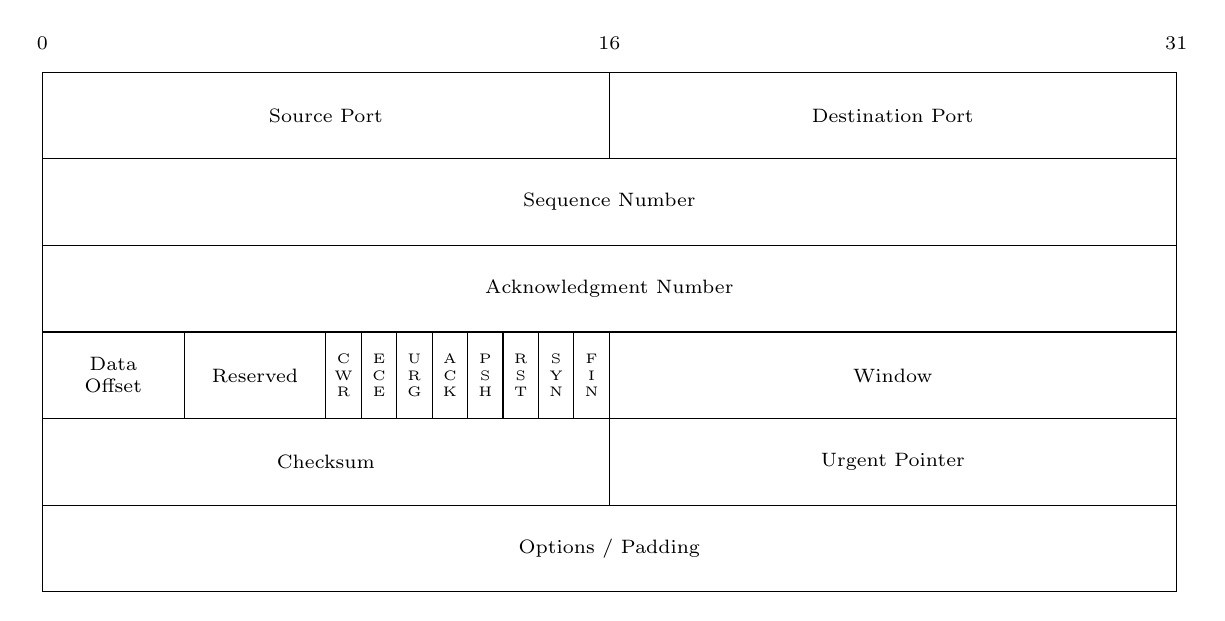
\begin{tikzpicture}[x=0.45cm, y=1.1cm, every node/.style={font=\scriptsize, align=center}]
        % Bit indices - 10 entfernt
        \node[anchor=south] at (0,6.15) {0};
        \node[anchor=south] at (16,6.15) {16};
        \node[anchor=south] at (32,6.15) {31};

        % Row 1: Source / Destination Port
        \draw (0,6) rectangle (16,5) node[midway] {Source Port};
        \draw (16,6) rectangle (32,5) node[midway] {Destination Port};

        % Row 2: Sequence Number
        \draw (0,5) rectangle (32,4) node[midway] {Sequence Number};

        % Row 3: Acknowledgment Number
        \draw (0,4) rectangle (32,3) node[midway] {Acknowledgment Number};

        % Row 4: Offset, Reserved, Flags, Window
        % Data Offset (4 Bits: 0-3)
        \draw (0,3) rectangle (4,2) node[midway] {Data\\Offset};
        
        % Reserved (4 Bits: 4-7) - "Rsrvd" wie in Vorlage
        \draw (4,3) rectangle (8,2) node[midway] {Reserved};

        % Flags (8 Bits: 8-15) - Einzelne Kästchen mit tiny Schrift gestapelt
        \draw (8,3) rectangle (9,2) node[midway, font=\tiny, inner sep=0pt] {C\\W\\R};
        \draw (9,3) rectangle (10,2) node[midway, font=\tiny, inner sep=0pt] {E\\C\\E};
        \draw (10,3) rectangle (11,2) node[midway, font=\tiny, inner sep=0pt] {U\\R\\G};
        \draw (11,3) rectangle (12,2) node[midway, font=\tiny, inner sep=0pt] {A\\C\\K};
        \draw (12,3) rectangle (13,2) node[midway, font=\tiny, inner sep=0pt] {P\\S\\H};
        \draw (13,3) rectangle (14,2) node[midway, font=\tiny, inner sep=0pt] {R\\S\\T};
        \draw (14,3) rectangle (15,2) node[midway, font=\tiny, inner sep=0pt] {S\\Y\\N};
        \draw (15,3) rectangle (16,2) node[midway, font=\tiny, inner sep=0pt] {F\\I\\N};

        % Window (16 Bits: 16-31)
        \draw (16,3) rectangle (32,2) node[midway] {Window};

        % Row 5: Checksum, Urgent Pointer
        \draw (0,2) rectangle (16,1) node[midway] {Checksum};
        \draw (16,2) rectangle (32,1) node[midway] {Urgent Pointer};

        % Row 6: Options / Padding
        \draw (0,1) rectangle (32,0) node[midway] {Options / Padding};
    \end{tikzpicture}
    \caption{Aufbau des TCP-Headers nach RFC 9293 \cite{Eddy_2022}.}
    \label{fig:tcp_header}
\end{figure}

Da das TCP-Protokoll Daten als \eng{Stream} statt einzeln (\eng{Message}) versendet, 
wird vorher eine Verbindung in einem sogenannten \eng{Three-Way-Handshake} aufgebaut \cite{Wendzel_2021} S71/72. 
Bei diesem werden TCP-Pakete mit jeweils unterschiedlichen Werten in den \eng{Control Bits} (\eng{Flags}) 
des TCP-Headers nach dem in \ref{fig:tcp_handshake} beschriebenen Muster ausgetauscht.

\begin{figure}[htbp]
    \centering
    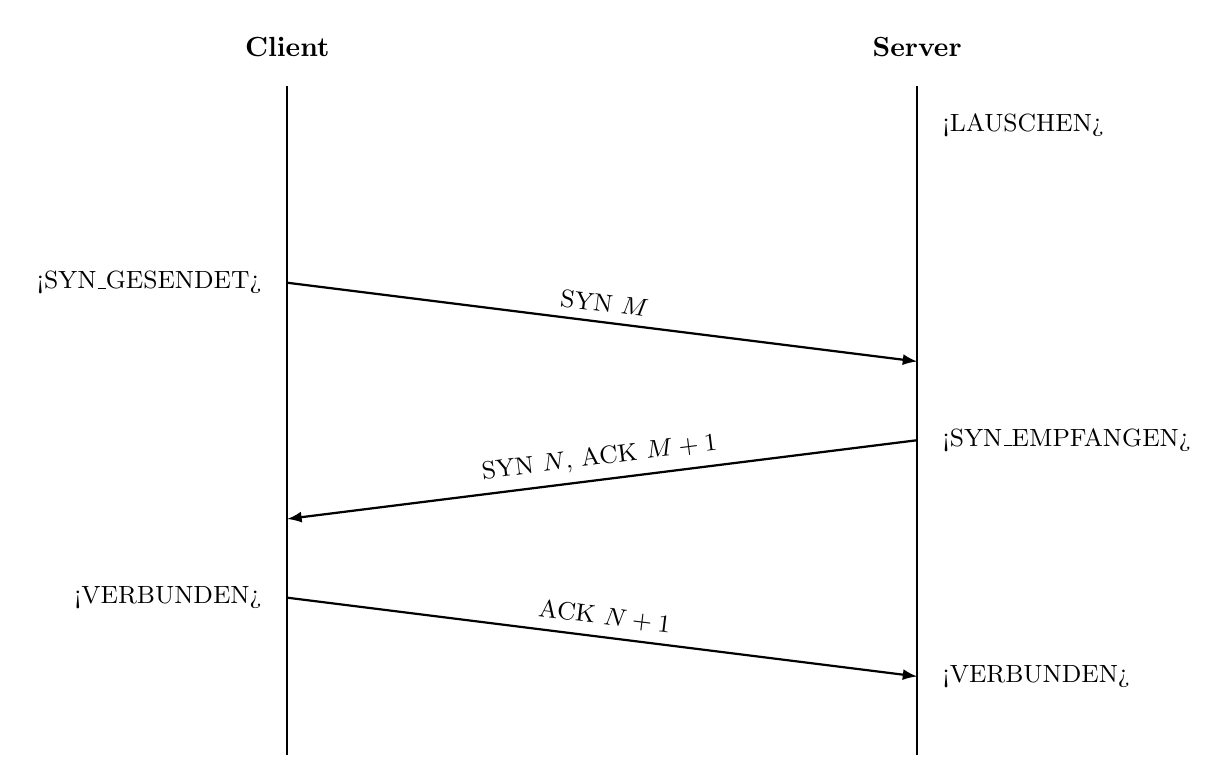
\begin{tikzpicture}[
        >=latex, 
        font=\small,
        node distance=1cm,
        every node/.style={align=center}
    ]

        % --- Koordinaten-Definition ---
        % X-Positionen der Linien
        \def\clientx{0}
        \def\serverx{8}
        
        % Y-Positionen der Ereignisse
        \def\yStart{0}
        \def\yListen{-0.5}
        \def\yConnect{-2}
        \def\ySynSend{-2.5}
        \def\ySynRecv{-3.5}
        \def\ySynAckSend{-4.5}
        \def\ySynAckRecv{-5.5}
        \def\yAckSend{-6.5}
        \def\yAckRecv{-7.5}
        \def\yEnd{-8.5}

        % --- Vertikale Linien (Timelines) ---
        \draw[thick] (\clientx, \yStart) -- (\clientx, \yEnd);
        \draw[thick] (\serverx, \yStart) -- (\serverx, \yEnd);

        % --- Header ---
        \node[font=\bfseries] at (\clientx, 0.5) {Client};
        \node[font=\bfseries] at (\serverx, 0.5) {Server};

        % --- SERVER SEITE (Rechts) ---
        % LISTEN Zustand
        \node[anchor=west] at (\serverx+0.2, \yListen) {<LAUSCHEN>};

        % SYN_RECV Zustand
        \node[anchor=west] at (\serverx+0.2, \ySynAckSend) {<SYN\_EMPFANGEN>};
        
        % ESTABLISHED Zustand
        \node[anchor=west] at (\serverx+0.2, \yAckRecv) {<VERBUNDEN>};


        % --- CLIENT SEITE (Links) ---
        % SYN_SENT Zustand
        \node[anchor=east] at (\clientx-0.2, \ySynSend) {<SYN\_GESENDET>};

        % ESTABLISHED Zustand
        \node[anchor=east] at (\clientx-0.2, \yAckSend) {<VERBUNDEN>};


        % --- NACHRICHTEN (Pfeile) ---
        
        % 1. SYN M
        \draw[->, thick] (\clientx, \ySynSend) -- (\serverx, \ySynRecv) 
            node[midway, above, sloped] {SYN $M$};

        % 2. SYN N, ACK M+1
        \draw[->, thick] (\serverx, \ySynAckSend) -- (\clientx, \ySynAckRecv) 
            node[midway, above, sloped] {SYN $N$, ACK $M+1$};

        % 3. ACK N+1
        \draw[->, thick] (\clientx, \yAckSend) -- (\serverx, \yAckRecv) 
            node[midway, above, sloped] {ACK $N+1$};

    \end{tikzpicture}
    \caption{\eng{Three-Way-Handshake} zum Aufbau einer TCP-Verbindung \cite{Wendzel_2021}.}
    \label{fig:tcp_handshake}
\end{figure}


\section{Portscanning} \label{Portscanning}
Portscanning, als Art des Netzwerkscannings, ist eines der fundamentalen Verfahren in der Netzwerksicherheit zum Auffinden von 
potenziellen Schwachstellen \cite{Chapter_4._Port_Scanning_Overview_|_Nmap_Network_Scanning}. Ein Portscanner verschickt Pakete an ein Zielsystem und
zieht anhand der Antworten, oder auch ausbleibenden Antworten, Rückschlüsse auf den Zustand des Systems. Das Ziel ist die Identifikation
von offenen Ports bzw. aktiven Diensten, was als erster Schritt für weiterführende Sicherheitsanalysen oder aber auch Angriffe dienen kann \cite[S.~4-3]{Scarfone_Souppaya_Cody_Orebaugh_2008}. 

Beim Scannen von Ports können grundsätzlich zwei strategische Ausrichtungen unterschieden werden:
\begin{itemize} 
	\item \textbf{Vertikales Scannen:} Hierbei wird ein einzelner Ziel-\eng{Host}\footnote{Teilnehmer im Netzwerk, der über eine IP-Adresse adressierbar ist.} 
    auf eine Vielzahl von Ports (oft alle 65535) gescannt, um ein möglichst
vollständiges Profil möglicher Schwachstellen des Zielsystems zu erlangen und somit eher für das \eng{Penetration Testing} geeignet ist.
\item \textbf{Horizontales Scannen:} Ein sehr großer Adressbereich, beispielsweise das komplette IPv4-Internet wird gescannt. Dafür ist die Anzahl
der zu scannenden Ports sehr klein oder auf einen einzigen beschränkt. Dies bietet die Möglichkeit wertvolle Daten über Trends oder
die Verbreitung von Schwachstellen zu untersuchen \cite{Durumeric_Wustrow_Halderman}.
\end{itemize} 

% bis hier Rechtschreibung kontrolliert

\subsection{SYN-Scanning}
Für einen \eng{Half-Open} \texttt{SYN}-Scan wie er in dieser Arbeit behandelt wird, sind lediglich die ersten beiden Schritte des in \ref{fig:tcp_handshake} 
dargestellten Verbindungsablaufes relevant. Es wird davon gebraucht gemacht, dass bereits und ausschließlich eine \texttt{SYN/ACK}-Antwort den Port als offen klassifiziert, 
was den weiteren Verbindungsaufbau irrelevant macht \cite{Lyon_2010}. Um den Scan zu verschleiern und den Verbindungsversuch trotz dessen sauber
abzuschießen, kann anschließend noch ein Paket, bei welchem die \texttt{RST}-Flag der \eng{Control Bits} gesetzt ist gesendet werden \cite{Lyon_2010}.

Um antwortende \eng{Hosts} effizient zu identifizieren, wird das Prinzip des \texttt{SYN}-Cookies adaptiert \cite{Durumeric_Wustrow_Halderman}, welches ursprünglich als 
Abwehrmechanismus gegen \eng{Denial-of-Service}-Angriffe spezifiziert wurde \cite[S. 8]{Eddy_2007}. Dafür werden verbindungsspezifische 
Informationen unter Verwendung eines \eng{Hash}-Algorithmus (z. B. \eng{Keyed SipHash} TODO opt. Quelle) kodiert 
und als \eng{Sequence Number} in den TCP-Header des ausgehenden \texttt{SYN}-Pakets eingetragen.
Antwortet ein Ziel-\eng{Host} mit einem \texttt{SYN-ACK}-Paket, so enthält dessen \eng{Acknowledgment Number} gemäß TCP-Spezifikation den inkrementierten 
Wert der ursprünglichen \eng{Sequence Number}. Die Validierung lässt sich abstrahiert wie folgt beschreiben:

\begin{verbatim}is_valid = hash(value_0, value_1, ..., secret) == answer.ack_num - 1\end{verbatim} \label{equ:syn_cookie_auswertung}

Die Validierung der Antwort erfolgt somit rein mathematisch und benötigt keine Speicherung in einer lokalen
Zustandstabelle. Dies erwirkt eine sowohl zeitliche als auch logische Entkopplung von Sende- und Empfangsprozessen,
was wiederum eine asynchrone Architektur ermöglicht.

Entscheidend für den Scanner sind demnach die in \ref{tab:TCP-header-fields} aufgeführten Header Felder. 

\begin{table}[htbp]
\begin{tabularx}{\textwidth}{|c|X|}\hline 
\textbf{Header Feld} & \textbf{Beschreibung} \\ \hline
\eng{Source Port} & Beschreibt den genutzten Port des Ausgangsdienstes. \\ \hline
\eng{Destination Port} &  Beschreibt den zu scannenden Port des Zielsystems. \\ \hline
\eng{Sequence Number} & Wird zur Speicherung des \texttt{SYN}-Cookies genutzt. \\ \hline
\eng{Acknowledgement Number} & Wird zum Abrufen des \texttt{SYN}-Cookies genutzt. \\ \hline
\eng{Control Bits} (\eng{Flags}) & Wird für die verschiedenen Phasen des Verbindungsaufbaues angepasst oder ausgelesen.  \\ \hline
\end{tabularx}
\label{tab:TCP-header-fields}
\caption{Relevante TCP-Header Felder}
\end{table}

\section{Schnittstellen zur Paketverarbeitung unter Linux}
Um einen performanten Scanner zu bauen, müssen die genutzten Technologien zum einen für die Netzwerkprogrammierung 
geeignet und zum anderen hohe Sende- und Empfangsraten zulassen, während möglichst wenig
Rechenressourcen verbraucht werden. 

\subsection{Linux}
Linux ist ein \eng{Open-Source}-Betriebssystem-Kernel \cite[S.~1]{Kerrisk_2018}, welcher aufgrund neuartiger Subsysteme (wie beispielsweise \texttt{eBPF} (siehe \ref{Grundlagen.eBPF}) oder
 \texttt{XDP} (siehe \ref{Grundlagen.XDP})), eine programmierbare Paketverarbeitung nahe an der Hardware ermöglicht. 
 Dies ist für die Entwicklung eines Hochleistungsscanners von großem Vorteil.

Ein zentrales Konzept zum Verständnis der \eng{Performance}-Grenzen ist die Unterscheidung 
zwischen \eng{User Space} und \eng{Kernel Space} im Linux Ökosystem \cite[S.~23]{Kerrisk_2018}: 

\begin{itemize} 
	\item \textbf{\eng{Kernel-Space}:} Hier läuft der Kern des Betriebssystems mit vollem Zugriff 
	auf die Hardware und den Speicher. Treiber und der Netzwerk-Stack operieren auf dieser Ebene. 
	\item \textbf{\eng{User-Space}:} Hier laufen reguläre Anwendungen in isolierten Speicherbereichen. 
	Diese haben keinen direkten Zugriff auf den \eng{Kernel Space}. 
\end{itemize} 
Die Kommunikation zwischen diesen Ebenen erfolgt über \eng{System Calls} \cite[S.~44]{Kerrisk_2018}. Jeder Wechsel (\eng{Context Switch}) 
zwischen \eng{User}- und \eng{Kernel Space}, sowie das Kopieren von Daten zwischen diesen 
Speicherbereichen, erzeugt \eng{Overhead}. Beim Versenden und Empfangen sehr vieler Pakete 
summiert sich dieser \eng{Overhead}, da jedes Paket im Normalfall sowohl \eng{Kernel Space}, als auch \eng{User Space}, 
durchschreitet. Dies belastet die CPU und wird für den Durchsatz zum Flaschenhals \cite{Høiland-Jørgensen_Brouer_Borkmann_Fastabend_Herbert_Ahern_Miller_2018}.

\subsection{\eng{Raw-Sockets} und \eng{Address Families}}
Als Endpunkt für die Kommunikation werden \eng{Sockets} genutzt \cite{socket2_linux_manpage}. Die traditionelle 
Netzwerkprogrammierung unter Linux abstrahiert die Komplexität der Netzwerkprotokolle wie TCP. So übernimmt der Kernel
dabei vollständig den \eng{Three-Way-Handshake} und die Zustandsverwaltung \cite[S.~1158]{Kerrisk_2018}. 
Für einen \texttt{SYN}-Scanner ist dies ungeeignet, da der Scanner lediglich das initiale \texttt{SYN}-Paket senden und die Antwort 
registrieren will, ohne eine vollwertige Verbindung aufzubauen, welche Ressourcen im Kernel binden würde.

\eng{Raw-Sockets} erlauben der Anwendung, Netzwerkpakete unter Umgehung bestimmter \eng{Layer} des Kernel-Stacks zu senden 
und zu empfangen \cite{raw7_linux_manpage}. Der Entwickler muss die Protokoll-Header selbst konstruieren. 
Dies ist für \eng{Half-Open} Portscanner essenziell, um individuelle Pakete zu generieren, ohne dass der Kernel 
automatisch in den Verbindungsaufbau eingreift. 

% TODO eindeutschen
Die \eng{Address Families} definieren dabei die Interpretation der Adressen und die Ebene des Zugriffs \cite{address_families7_linux_manpage}. 
Der Linux-Kernel stellt diverse Address-Familien bereit. Zum Verständnis, im Rahmen dieses Projektes, sind folgende Varianten von zentraler 
Bedeutung:

\begin{itemize} 
	\itemsep 0pt
	\item \textbf{\texttt{AF\_INET} (Netzwerk-Ebene):} Diese Familie operiert auf Layer 3 der IP-Ebene \cite{raw7_linux_manpage}. Bei Nutzung von \eng{Raw-Sockets} fügt der Kernel 
    standardmäßig den IP-Header hinzu und übernimmt das vollständige Routing zur korrekten Netzwerkschnittstelle \cite[S.~1202]{Kerrisk_2018}.
 	\item \textbf{\texttt{AF\_PACKET} (Sicherungsschicht):} Diese Familie ermöglicht direkten Zugriff auf Layer 2 (Ethernet-Ebene). 
	Anwendungen erzeugen vollständige \eng{Ethernet-Frames} und haben somit die volle Kontrolle.
    Das Versenden oder Empfangen von Paketen erfordert jedoch weiterhin die Allokation von Kernel-internen Datenstrukturen \cite{packet_7_-_Linux_manual_page}.
    \item \textbf{\texttt{AF\_XDP} (Hochperformant):} Hierbei handelt es sich um eine speziell für Hochleistungsanwendungen optimierte \eng{Address Family}.
	Sie ermöglicht das Senden und Empfangen von Paketen unter Umgehung des regulären Kernel-Netzwerkstacks. Dabei ist zwischen dem universell verfügbaren \eng{Copy-Mode},
    in welchem Daten zwischen Kernel und User Space kopiert werden und dem Treiber-abhängigen \eng{Zero-Copy-Mode}, in welchem Daten direkt in den Speicher der 
    Anwendung geschrieben werden zu unterscheiden \cite{Høiland-Jørgensen_Brouer_Borkmann_Fastabend_Herbert_Ahern_Miller_2018}. 
\end{itemize}

\subsection{Erweiterte Berkeley Packet Filter (\texttt{eBPF})} \label{Grundlagen.eBPF}
Ursprünglich als \textit{Berkeley Packet Filter} (\texttt{BPF}) für Werkzeuge wie \texttt{tcpdump} entwickelt, um Pakete effizient zu filtern \cite{260309}, 
wurde die Technologie erweitert, sodass grundlegend neue Möglichkeiten außerhalb des reinen filtern von Paketen erschlossen wurden. 

\texttt{eBPF} ist eine im Linux-Kernel integrierte virtuelle Maschine (VM), die es erlaubt, benutzerdefinierten 
\eng{Bytecode} sicher und effizient im \eng{Kernel}-Kontext (siehe \ref{fig:rx_xdp}) auszuführen, ohne Kernel-Module schreiben oder den Kernel 
neu kompilieren zu müssen \cite{Nishanth_Reddy_Pinnapareddy_2025}. \texttt{eBPF}-Programme werden zur Laufzeit 
durch einen \eng{JIT-Compiler} (\eng{Just-In-Time}) in native Maschinensprache übersetzt. Ein \eng{Verifier} stellt 
vor der Ausführung sicher, dass der Code sicher ist \cite{Vieira_Castanho_Pacífico_Santos_Júnior_Vieira_2021}. 
So werden Fehler wie beispielsweise Endlosschleifen oder falsche Speicherzugriffe vermieden.

Da eBPF-Programme ereignisbasiert ausgeführt werden und keinen eigenen persistenten Speicher besitzen, 
werden sogenannte \texttt{bpf} Maps verwendet, um Zustände zu bewahren und Daten auszutauschen \cite{Høiland-Jørgensen_Brouer_Borkmann_Fastabend_Herbert_Ahern_Miller_2018}. 
Dies sind generische \eng{Key-Value}-Speicher, die sowohl von verschiedenen eBPF-Programmen 
als auch vom \eng{User Space} gelesen und beschrieben werden können \cite{Høiland-Jørgensen_Brouer_Borkmann_Fastabend_Herbert_Ahern_Miller_2018}.
Dabei gibt es verschiedene Datenstrukturen. Eine davon ist der \texttt{RingBuf} 
(\texttt{BPF\_MAP\_TYPE\_RINGBUF}). Hierbei handelt es sich um einen für den Datenaustausch 
vom Kernel zum \eng{User Space} optimierten Ringpuffer, der 
im Vergleich zu älteren Methoden wie \eng{Perf Buffer} durch geteilte Speicherregionen effizienter arbeitet 
und die Reihenfolge der Ereignisse garantiert \cite{Map_Type_“BPF_MAP_TYPE_RINGBUF”_-_eBPF_Docs}.

Für einen \texttt{SYN}-Scanner ist \texttt{eBPF} nützlich, da es ermöglicht, eingehende Antwortpakete (\texttt{SYN-ACK}) extrem früh 
zu filtern und an den \eng{User Space} weiterzuleiten, bevor teure Speicherstrukturen des Kernels angelegt werden. 
So werden nur relevante Daten an den \eng{User Space} weitergereicht. 

\subsection{eXpress Data Path (\texttt{XDP})} \label{Grundlagen.XDP}
\texttt{XDP} definiert eine limitierte Ausführungsumgebung für \texttt{eBPF}-Programme, die direkt im Kontext des 
Netzwerktreibers ausgeführt werden.
Dies ermöglicht eine programmierbare und hochperformante Paketverarbeitung direkt im Betriebssystemkern. 
Im Gegensatz zu früheren Ansätzen, die den Kernel vollständig umgehen (z.B. \texttt{DPDK}), 
integriert sich \texttt{XDP} kooperativ in den bestehenden Stack. \cite{Høiland-Jørgensen_Brouer_Borkmann_Fastabend_Herbert_Ahern_Miller_2018} 

Ein \texttt{XDP}-Programm kann Pakete verwerfen (\texttt{XDP\_DROP}), an den regulären Netzwerkstack weiterleiten (\texttt{XDP\_PASS}), 
über dieselbe Schnittstelle zurücksenden (\texttt{XDP\_TX}) oder an eine andere CPU bzw. einen \eng{Userspace-Socket} 
umleiten (\texttt{XDP\_REDIRECT}) \cite{Høiland-Jørgensen_Brouer_Borkmann_Fastabend_Herbert_Ahern_Miller_2018}\cite{Vieira_Castanho_Pacífico_Santos_Júnior_Vieira_2021}.

Die Effizienz von \texttt{XDP} resultiert aus der Positionierung im Datenpfad. In herkömmlichen 
Linux-Netzwerkarchitekturen durchläuft ein Paket nach dem Empfang durch die Netzwerkkarte den 
gesamten Netzwerk-Stack. Erst danach erreichen die Daten den \eng{User Space}. Dies erfordert CPU und Speicher-
aufwendige \eng{Context Switches} (\eng{Context Switches}) zwischen \eng{Kernel-} und \eng{User-Mode}, sowie die Allokation 
komplexer Metadatenstrukturen (eines \texttt{sk\_buff} \footnote{\eng{Socket Buffer}}) \cite{Høiland-Jørgensen_Brouer_Borkmann_Fastabend_Herbert_Ahern_Miller_2018}\cite{Zhang_Shu_Chen_Xie_2024}.
\texttt{XDP} greift vor dieser Allokation ein (siehe Abbildung \ref{fig:rx_xdp}). Tests zeigen, dass \texttt{XDP} auf einem einzelnen CPU-Kern bis zu 
fünfmal mehr Pakete pro Sekunde verarbeiten kann als der Standard Linux-Stack \cite{Høiland-Jørgensen_Brouer_Borkmann_Fastabend_Herbert_Ahern_Miller_2018}.

% TODO Pfeil vom ebpf Programm muss orange sein
\begin{figure}[htbp]
	\centering
	\includegraphics[width=\textwidth]{pictures/RX_Kernel_hell_3.drawio.png}
	\caption{Der Empfangspfad durch den Kernel bei der Nutzung von \texttt{XDP} und \texttt{eBPF} (vereinfacht). Orientiert an Høiland et al. \cite{Høiland-Jørgensen_Brouer_Borkmann_Fastabend_Herbert_Ahern_Miller_2018}.}
	\label{fig:rx_xdp}
\end{figure}

Die \eng{Performance} und Verfügbarkeit von \texttt{XDP} hängen vom verwendeten Betriebsmodus ab. 
Nach Zhang et al. \cite{Zhang_Shu_Chen_Xie_2024} und Vieira et al. \cite{Vieira_Castanho_Pacífico_Santos_Júnior_Vieira_2021} 
lassen sich drei Modi unterscheiden:

\begin{itemize} 
	\item \textbf{\eng{Native Mode} (\eng{Driver Mode}):} Dies ist der Standardmodus für Hochleistungsanwendungen. 
	Das \texttt{XDP}-Programm wird direkt im Netzwerkkartentreiber ausgeführt. Die Verarbeitung erfolgt nach dem 
	\eng{DMA}-Transfer (\eng{Direct Memory Access}) in den \eng{Ring-Buffer}, aber vor der \texttt{sk\_buff}-Allokation. 
	Dies erfordert explizite Unterstützung durch den Treiber der Netzwerkkarte. 
	\item \textbf{\eng{Offloaded Mode} (\eng{Hardware Mode}):} Hierbei wird das \texttt{eBPF}-Programm vom Kernel auf die 
	Netzwerkkarte ausgelagert und direkt auf der Hardware ausgeführt. Dies bietet die höchste 
	\eng{Performance}, da die Host-CPU vollständig von der Paketverarbeitung entlastet wird, setzt aber
	die Nutzung einer sogenannten \eng{Smart NIC} Netzwerkkarte voraus. 
	\item \textbf{\eng{Generic Mode} (\eng{SKB Mode}):} Dieser Modus dient der Kompatibilität. Wenn ein Treiber \texttt{XDP} 
	nicht nativ unterstützt, führt der Kernel das \texttt{XDP}-Programm im Netzwerkstack des Kernels
	aus. Zwar gehen hier die massiven \eng{Performance}-Vorteile der Speicherersparnis verloren, 
	jedoch wird sichergestellt, dass \texttt{XDP}-Anwendungen auf jeder Hardware funktionsfähig bleiben. 
\end{itemize}

\section{Die Programmiersprache: Rust} \label{rust}
Rust ist eine multiparadigmatische Systemprogrammiersprache, die ursprünglich von Mozilla Research entwickelt wurde.
Der Hauptfokus der Sprache ist die Sicherheit. Doch auch \eng{Performance} und Nebenläufigkeit sind immer weiter in 
den Fokus gerückt \cite{Bugden_Alahmar_2022}. Dabei schafft es Rust als erste Sprache
Speichersicherheits-Konzepte von Sprachen hoher Abstraktionsebene mit der Entscheidungsfreiheit 
über die Ressourcenverwaltung von Sprachen niedriger 
Abstraktionsebene zu vereinen \cite{Jung_Jourdan_Krebbers_Dreyer_2021}.

\subsection{Konzepte und Besonderheiten}
Sprachen hoher Abstraktionsebene bedienen sich häufig einer automatisierten Speicherverwaltung mithilfe eines 
\eng{Garbage Collectors}, um Speicherfehler, welche das Sicherheitsniveau einer Sprache maßgeblich 
bestimmen \cite{bugden2022safety}, zu vermeiden. Rust hingegen nutzt ein einzigartiges Modell, welches 
durch drei zentrale Konzepte bestimmt wird:

\begin{itemize} \label{rust.concepts}
	\item \textbf{\eng{Ownership}:} Jede Variable hat einen \eng{Owner} (Besitzer). Wird der Besitzer gelöscht,
	wird auch die Variable gelöscht. Die Variable kann nur einen Besitzer haben \cite{RustBelt}. Das bewirkt,
	dass der Programmierer sich nicht um das Freigeben des Speichers kümmern muss.
	\item \textbf{\eng{Borrowing}:} Um eine Variable als Referenz in mehreren Kontexten nutzen zu können, 
	ohne dessen \eng{Owner} zu wechseln, gibt es das \eng{Borrowing} Konzept, mit folgenden Regeln:
	es kann entweder eine veränderbare oder mehrere unveränderbare Referenzen einer Variable 
	geben \cite{Bugden_Alahmar_2022}. 
	\item \textbf{\eng{Lifetimes}:} Jede Referenz in Rust besitzt eine Lebensdauer (\eng{Lifetime}), 
    welche den Gültigkeitsbereich definiert, in dem die Referenz valide ist. Meist implizit vom Compiler abgeleitet, 
    verhindern \eng{Lifetimes} falsche Zugriffe, indem sie sicherstellen, dass die referenzierten 
    Daten mindestens so lange existieren wie die Referenz selbst \cite{Bugden_Alahmar_2022}.
\end{itemize}

Die Einhaltung dieser Regeln wird zur Kompilierzeit vom \eng{Borrow-Checker} verifiziert. 
Außerdem hat Rust noch weitere Konzepte zur Steigerung der Sicherheit. 
Budgen et al. \cite{Bugden_Alahmar_2022} führen weitere Konzepte wie das
\eng{Bounds Checking}, welches auf ungültige Indexzugriffe prüft oder 
die Nutzung von \texttt{Option}s, welche Zugriffe auf nicht initialisierte Werte vermeiden, indem
sie eine Struktur, welche entweder den gewünschten Wert x als \texttt{Some(x)} oder \texttt{None} enthält, zurückgeben auf. 
Außerdem muss \eng{Pointer}-Arithmetik in sogenannte \texttt{unsafe}-Blöcke ausgelagert werden.
Diese dienen als eine Art Umgehungsmöglichkeit der anderen Konzepte. Sie lösen
im Fehlerfall eine Programm-beendenden \texttt{panic} aus, welche verhindert, dass das Programm
in einem undefinierten Zustand weiter läuft.

Trotz der Möglichkeit und Notwendigkeit, \texttt{unsafe}-Blöcke zu nutzen (beispielsweise für hardwarenahe
Operationen oder der Arbeit mit C-Bibliotheken), was dem Sicherheitskonzept der Sprache
widerspricht, sind laut Jung et al. \enquote{zahlreiche wichtige Rust Bibliotheken} \cite{RustBelt}
sicher, da sie die \texttt{unsafe}-Blöcke korrekt kapseln \cite{RustBelt}.

Durch das Zusammenspiel dieser Konzepte können Speicherfehler verschiedenster Art 
bereits zur Kompilierzeit vermieden werden, was Rust zur sichersten unter den derzeit
gängigen Sprachen macht \cite{bugden2022safety}. Allerdings müssen deshalb auch einige
Regeln bei der Programmierung beachtet und eingehalten werden, weshalb der Sprache eine 
steile Lernkurve zugeschrieben wird \cite{Cui_Xu_2025}.

\subsection{Asynchrone Programmierung und \eng{Performance} von Rust}
Die im letzten Abschnitt genannten Konzepte schließen auch \eng{Data Races}, 
welche beim Zugriff mehrerer \eng{Threads} \footnote{Untergeordnete Arbeitseinheiten eines Prozesses} auf 
den gleichen Speicher entstehen können, bereits zur Kompilierzeit aus \cite{Costanzo_Rucci_Naiouf_Giusti_2021}. 
Dies macht \eng{Data Races} zu einer häufigen Fehlerquelle in der asynchronen Programmierung \cite{Bugden_Alahmar_2022}.
Die Beseitigung derer, macht Rust zu einer guten Wahl für sowohl nebenläufige als auch parallele Programmierung. 

\subsubsection{Nebenläufige und Parallele Programmierung}
Die nebenläufige Programmierung, welche in Rust durch das 
\texttt{async/await}-Modell umgesetzt wird, befasst sich mit der logischen Strukturierung von Software 
in unabhängige Kontrollflüsse. Diese agieren zeitlich verschränkt, wobei der primäre Zweck nicht 
die gleichzeitige Ausführung, sondern die Entkopplung von Aufgaben ist. So werden Ressourcen effektiv genutzt,
indem sie während möglicher Wartezeiten z.B. bei \eng{I/O}-Operationen\footnote{Input-/Output-Operationen}, für andere
Prozesse freigegeben werden. Dadurch kann die Effizienz und die Responsivität des Systems erhöht werden \cite{Silberschatz_Galvin_Gagne_2018} \cite{Arpaci-Dusseau_Arpaci-Dusseau_2018}.

Die Parallelität hingegen, bezieht sich auf die tatsächliche physikalische Ausführung mehrerer 
Aufgaben zum gleichen Zeitpunkt \cite{Silberschatz_Galvin_Gagne_2018}, was eine entsprechende \eng{Multi-Core}-Hardware voraussetzt \cite{Concurrency_is_not_parallelism_-_The_Go_Programming_Language}. 
Der Vorteil der Parallelität liegt in der Leistungssteigerung und der Maximierung des 
Datendurchsatzes bei rechenintensiven Problemen \cite{Silberschatz_Galvin_Gagne_2018}\cite{Arpaci-Dusseau_Arpaci-Dusseau_2018}.

\subsubsection{Rusts Konzepte zur \eng{Performance}-Steigerung}
Neben den möglichen \eng{Performance}-Vorteilen durch die nebenläufige Programmierung, welche
aber letztendlich dem Programmierer überlassen ist, bietet die Sprache ihre 
größten internen \eng{Performance}-Vorteile durch die \eng{Zero-Cost Abstraction}. 
Das Konzept der \eng{Zero-Cost Abstraction} \cite{Cui_Xu_2025}, welches auch in der Sprache C++ Anwendung
findet, kann nach Bjarne Stroustrup wie folgt beschrieben werden: \enquote{Was man nicht 
nutzt, dafür bezahlt man nicht. Was man nutzt, könnte man selbst nicht 
besser per Hand codieren} \cite{Stroustrup_1994}.

Dazugehörige Konzepte sind beispielsweise die Eliminierung von Laufzeit-\eng{Overhead} durch 
die Vermeidung eines zur Laufzeit arbeitenden \eng{Garbage Collectors} \cite{bugden2022safety} \cite{Cui_Xu_2025}, 
die \textit{Monomorphisierung} um die Typen oder Größen generischer Strukturen wie z.B.
\texttt{Vec} \footnote{Vektor, ähnlich einer Liste} oder \texttt{Option} nicht mehr während der Laufzeit 
bestimmen zu müssen \cite{Cui_Xu_2025}, oder die Bereitstellung eigener Iteratoren, welche 
die Leistung manuell geschriebener Schleifen oft übertrifft \cite{Cui_Xu_2025}.

Diese Konzepte und vor allem die Prüfung der in \ref{rust.concepts} vorgestellten Konzepte zur 
Kompilierzeit, führt dazu, dass Rust in Benchmarks gängige Sprachen wie Java, Python,
oder Go übertrifft und sogar mit der Geschwindigkeit von C konkurriert \cite{Costanzo_Rucci_Naiouf_Giusti_2021}
\cite{Bugden_Alahmar_2022} \cite{Cui_Xu_2025}.
% !TEX root = ../Thesis.tex
%%
%%  Hochschule für Technik und Wirtschaft Berlin --  Abschlussarbeit
%%
%% Kapitel 3 - Methodik und Anforderungsanalyse
%%
%%

\chapter{Stand der Technik} \label{Stand_der_Technik}
In diesem Kapitel wird im ersten Schritt die historische Entwicklung des horizontalen Netzwerkscannings betrachtet.
Daraufhin werden in der Forschung etablierte Scanner sowie alternative Ansätze vorgestellt, diskutiert und
die resultierenden Nachteile betrachtet. 
Es folgt ein kurzer Überblick über weitere relevante Forschungsarbeiten zu relevanten Forschungssträngen
sowie die Auswahl der Scanner, welche später als Vergleichsobjekte dienen.

\section{Historische Entwicklung des horizontalen Netzwerkscannings} \label{Ch3_Historische_Entwicklung}
Ursprüngliche Netzwerkscanner wie Nmap \cite{Lyon_2010} wurden primär für die vertikale Analyse einzelner \eng{Hosts} oder 
kleiner Netzwerke konzipiert. Sie arbeiten teils zustandsbehaftet, was bedeutet, dass für jede 
ausgesendete Anfrage ein eigener Eintrag im Arbeitsspeicher verwaltet wird, um den Verbindungsstatus abzubilden. 
Bei Internet-weiten Scans führt dieser Ansatz jedoch schnell zur Erschöpfung der Systemressourcen und limitiert die 
Scan-Geschwindigkeit drastisch. Ein vollständiger Scan des Internets benötigte mit diesen Methoden 
oft Wochen oder Monate \cite{Durumeric_Wustrow_Halderman}.

Der entscheidende Durchbruch gelang 2013 mit der Veröffentlichung von ZMap durch Durumeric et al. 
Mithilfe eines radikalen Architekturwechsels hin zum zustandslosen Scanning 
konnte die Geschwindigkeit soweit gesteigert werden, dass 97\,\% der theoretischen Geschwindigkeit 
von Gigabit-Ethernet erreicht wurden. Dies ermöglichte erstmals Scans des gesamten IPv4-Adressraums 
in unter 45 Minuten von einem einzelnen Rechner aus \cite{Durumeric_Wustrow_Halderman}. Spätere Arbeiten, wie 
Zippier ZMap, optimierten diesen Ansatz weiter, um auch bis zu 10-Gbps-Leitungen auszulasten \cite{Adrian_Durumeric_Singh_Halderman}
und somit die anhaltende Relevanz des ZMap-Projektes zu unterstreichen.

\subsection{Der Standard Scanner: ZMap} \label{Ch3_S1_ZMap}
In der wissenschaftlichen Literatur gilt ZMap \cite{Durumeric_Wustrow_Halderman} als der De-facto-Standard und als das primäre Vergleichsobjekt für 
internetweite Scans. In einer Retrospektive aus dem Jahr 2024 stellen Durumeric et al. fest, dass ZMap die Art und Weise, wie Internetmessungen 
durchgeführt werden, fundamental verändert hat. Mit über 1.200 wissenschaftlichen Zitationen und der Nutzung als 
Basis für kommerzielle Sicherheitsanalysen (z.\,B. Censys) ist es das am weitesten verbreitete Werkzeug seiner Art \cite{Durumeric_Adrian_Stephens_Wustrow_Halderman_2024}.

Der Kern der Leistungsfähigkeit von ZMap lässt sich auf drei wesentliche Implementierungsentscheidungen zurückführen:

\begin{itemize} 
	\item \textbf{Effiziente \eng{I/O}-Schnittstellen:} ZMap nutzt standardmäßig \texttt{AF\_PACKET} in Kombination mit \eng{Memory Mapping} (\texttt{mmap}), 
    um den \eng{Overhead} des Kopierens zwischen Kernel und \eng{User-Space} zu reduzieren. Zwar zeigten Erweiterungen wie 
    Zippier ZMap \cite{Adrian_Durumeric_Singh_Halderman}, dass durch spezialisierte Treiber wie \texttt{PF\_RING ZC} (\eng{Zero-Copy}) 
    noch höhere Geschwindigkeiten möglich sind, jedoch weisen die Autoren darauf 
    hin, dass solche externen Treiber oft Wartungsprobleme und Inkompatibilitäten mit sich bringen. 
    Daher setzt die aktuelle Version von ZMap primär auf universell verfügbare Linux-Schnittstellen, 
    auch wenn diese \eng{Performance}-technisch limitiert sind \cite{Durumeric_Adrian_Stephens_Wustrow_Halderman_2024}.

    \item \textbf{Zustandslose Architektur:} ZMap nutzt das Prinzip der \texttt{SYN}-Cookies, um keinen Zustand 
    für ausgehende Verbindungen im Arbeitsspeicher halten zu müssen. 

    \item \textbf{Adressgenerierung mittels zyklischer Gruppen:} ZMap nutzt zyklische multiplikative Gruppen 
    modulo $p$ (wobei $p$ eine Primzahl $> 2^{32}$ ist). Dies ermöglicht eine pseudozufällige Permutation des gesamten 
    IPv4-Adressraums, was nötig ist, um Zielnetzwerke nicht zu überlasten. \cite{Durumeric_Wustrow_Halderman}.
\end{itemize}

\section{Alternative Implementierungsansätze} \label{Ch3_Alternative_Implementierungsansätze}
Neben der reinen \eng{Socket}-Programmierung und klassischen \eng{Raw-Sockets} haben sich weitere, teils modernere 
Techniken und Scanner-Architekturen aufgetan. Beispielsweise mithilfe von:

\begin{itemize} 
\item \textbf{\eng{Kernel-Bypass} mit \texttt{DPDK}:} Das Data Plane Development Kit (\texttt{DPDK}) erlaubt es Anwendungen, die Netzwerkkarte 
direkt aus dem \eng{User-Space} anzusprechen und den Kernel komplett zu umgehen. Abu Bakar und Kijsirikul zeigen, dass 
\texttt{DPDK}-basierte Scanner extrem hohe Raten erzielen können \cite{Abu_Bakar_Kijsirikul_2023}. Der Nachteil ist jedoch 
die hohe Komplexität, die exklusive Belegung von CPU-Kernen und die schwierige Integration in bestehende Systemumgebungen \cite{Høiland-Jørgensen_Brouer_Borkmann_Fastabend_Herbert_Ahern_Miller_2018}.

\item \textbf{Eigener TCP-Stack im \eng{User-Space} (Masscan):} Der Scanner Masscan \cite{Graham_2026} umgeht den Flaschenhals des Betriebssystems 
mithilfe eines eigenen TCP-Stacks im \eng{User-Space}. Dies erlaubt es dem Scanner, die Statusverwaltung und das Timing von Paketen 
komplett unabhängig vom Kernel-\eng{Scheduler} zu steuern. Der \eng{Scheduler} ist normalerweise dafür verantwortlich, die Rechenzeit der 
CPU auf die laufenden Prozesse zu verteilen \cite[S.~737]{Kerrisk_2018}. Die dabei entstehenden \eng{Context Switches} können das präzise Timing von Hochleistungsanwendungen 
stören. Dadurch kann Masscan deutliche \eng{Performance}-Gewinne gegenüber ZMap erreichen \cite{Pittman_2023}.

\item \textbf{\eng{Hardware-Offloading} und \eng{SmartNICs}:} Um die CPU des \eng{Host}-Systems zu entlasten, lagert IMap 
die Scan-Logik direkt auf die Netzwerkhardware aus. Durch den Einsatz von programmierbaren Switches oder \eng{SmartNICs} können Pakete 
bereits auf der Netzwerkkarte generiert und Antworten gefiltert werden, bevor sie überhaupt die CPU erreichen.
Dies erfordert jedoch spezialisierte Hardware.
In dieser Untersuchung wurde mit Raten von 40Gbps getestet, wobei jedoch Raten von einem Terabit oder mehr laut Li et al. theoretisch möglich wären. \cite{Li_Zhang_Guo_Bao_Xu_Hu_Li_2022}   
\end{itemize}

\section{Weitere relevante wissenschaftliche Arbeiten} \label{Ch3_Weitere_Arbeiten}
Der Forschungsstand zu horizontalen Hochleistungs-Netzwerkscannern wurde bereits in den vorherigen Abschnitten \cref{Ch3_Historische_Entwicklung,Ch3_Alternative_Implementierungsansätze} aufgegriffen. Ergänzend dazu ist noch anzubringen, dass nach bestehenden Ansätzen zur Kernel-Umgehung
die Arbeit zu \texttt{XDP} (\eng{eXpress Data Path}) einen Paradigmenwechsel darstellt. Zuvor genutzte Umgehungsstrategien waren unter anderem Netmap \cite{Rizzo}, 
welches bereits 2012 Konzepte wie \eng{Shared Memory}\footnote{Zwischen \eng{User-Space} und \eng{Kernel-Space} geteilter Speicher} 
und \eng{Zero-Copy} einführte, aber den Netzwerkstack eher ersetzte, statt ihn zu komplementieren, oder \texttt{DPDK} (siehe \cref{Ch3_Alternative_Implementierungsansätze}). 
Høiland-Jørgensen et al. zeigen, dass mit \texttt{XDP} durch eine programmierbare 
Paketverarbeitung im Kernel-Treiber eine mit \texttt{DPDK} vergleichbare \eng{Performance} erreicht werden kann, ohne die Integration in das Betriebssystem 
aufzugeben \cite{Høiland-Jørgensen_Brouer_Borkmann_Fastabend_Herbert_Ahern_Miller_2018}. 

Zwei Studien vergleichen \texttt{SYN}-Scanner \cite{Pittman_2023} \cite{Taupaani_Harwahyu_2025}, fokussieren sich aber eher auf die Trefferrate, welche in der Arbeit
nicht priorisiert wird (siehe \cref{Abgrenzung}). Außerdem ist die Gestaltung der Testumgebung bei beiden Arbeiten nicht auf Hochleistungs-Szenarien ausgelegt. 

Die Eignung von Rust für hochperformante Netzwerkprogrammierung wird in mehreren wissenschaftlichen Arbeiten evaluiert. Sagramoni et al.
schrieben eine Netzwerkbibliothek in Rust und verglichen sie mit der ursprünglichen C-Bibliothek \cite{Sagramoni_Lettieri_Procissi_2024}.
Gonzalez et al. entwickelten einen UDP Treiber für Linux und verglichen diesen mit einem ähnlichen C-Treiber \cite{Gonzalez2023Takeaways}.
Moon et al. erstellten einen \eng{NAT} (Network Address Translator) und testeten den Durchsatz \cite{Moon2017Toward}. 
Alle kommen zu dem Ergebnis, dass Rust sich für die \eng{Low-Level}-Netzwerkprogrammierung gut eignet und eine minimal niedrigere \eng{Performance}  
verglichen mit der aktuellen Standardsprache in diesem Bereich - C - aufweist. Emmerich et al. verglichen Rust mit
einer Vielzahl von anderen Sprachen, indem sie einen Netzwerktreiber in jeder der untersuchten Sprachen schrieben und 
diese anschließend miteinander verglichen. Dabei stellte sich Rust aufgrund seiner Sicherheitsgarantien und Performanz
als erste Wahl für zukünftige Treiber-Projekte heraus \cite{Emmerich_Ellmann_Bonk_Egger_Sánchez-Torija_Günzel_Di_Luzio_Obada_Stadlmeier_Voit_et_al._2019}.

Weitere Arbeiten beschäftigen sich mit dem Thema Sicherheit von Rust verglichen mit anderen Programmiersprachen und kamen zum
einheitlichen Ergebnis, dass Rust umfangreiche Sicherheitsgarantien mitbringt, die man so von keiner anderen gängigen Sprache
erhält \cite{Bugden_Alahmar_2022} \cite{bugden2022safety} \cite{Balasubramanian2017System}.

\section{Vergleichsobjekte für die Evaluation}
Um die Eignung der Implementierung in seiner Funktion als Performanz-orientierter \texttt{SYN}-Scanner aussagekräftig evaluieren zu können,
wird er im Evaluationsteil der Arbeit mit folgenden Scannern verglichen

\begin{itemize}
    \item \textbf{Wissenschaftlicher Standard:} Als primäres Vergleichsobjekt dient ZMap \cite{Durumeric_Wustrow_Halderman}, 
    da dieser die historische Basis des Internetscannings darstellt (siehe \cref{Ch3_S1_ZMap}). Da ZMap in C geschrieben ist und auf 
    klassischen Linux-Schnittstellen basiert, dient er als \eng{Baseline}, um zu untersuchen, ob die im Lösungsansatz gewählte Kombination 
    aus Rust und \texttt{XDP} trotz der Sicherheitsgarantien mit der etablierten Referenz konkurrieren kann.
    \item \textbf{Performance-Referenz:} Ergänzend wird Masscan \cite{Graham_2026} herangezogen. Dieser gilt durch seinen 
    eigenen \eng{User-Space}-Stack (siehe \cref{Ch3_Alternative_Implementierungsansätze}) als einer der schnellsten verfügbaren Scanner. 
    Dieser Vergleich ist sinnvoll, um die Effizienz der \texttt{XDP}-basierten Lösung gegenüber einem hochoptimierten C-Ansatz einzuordnen.
\end{itemize}

\section{Nachteile bisheriger Ansätze}
\subsection{Nachteile C-basierter Ansätze}
Obwohl ZMap und ähnliche Hochleistungsscanner (wie Masscan oder \texttt{DPDK}-Scanner) extrem effizient sind, 
basieren sie fast ausschließlich auf der Programmiersprache C. Diese technologische Monokultur bringt jedoch signifikante Nachteile mit sich.

Ein zentraler Nachteil ist die fehlende intrinsische Speichersicherheit von C \cite{van_Oorschot_2023}. Da die Sprache dem Entwickler die volle 
Verantwortung für die Speicherverwaltung überträgt, führen menschliche Fehler häufig zu schwerwiegenden Sicherheitslücken. 
Schwachstellen wie \eng{Buffer Overflows} in C/C++-basierten Systemen zählen nach wie 
vor zu den häufigsten Ursachen für Sicherheitslücken \cite{Al_Boghdady_Wassif_El_Ramly_2021}. 

Darüber hinaus geht die Leistungsfähigkeit von C oft zu Lasten der Wartbarkeit und Entwicklungseffizienz \cite{Costanzo_Rucci_Naiouf_Giusti_2021}. 
Um maximale Durchsatzraten zu erzielen, sind in C häufig komplexe, manuelle Optimierungen notwendig. Costanzo et al. heben
hervor, dass die Entwicklung von korrektem und effizientem C-Code im Vergleich zu Rust-Code
einen signifikant höheren Programmieraufwand erfordert, insbesondere wenn komplexe Nebenläufigkeit 
umgesetzt werden soll \cite{Costanzo_Rucci_Naiouf_Giusti_2021}. Selbst die Autoren von 
ZMap sagen in ihrer Retrospektive explizit, dass sie für eine heutige Implementierung ihres Scanners Rust 
wählen würden, um die Wartbarkeit und Sicherheit der Codebasis langfristig zu gewährleisten \cite{Durumeric_Adrian_Stephens_Wustrow_Halderman_2024}.

Ein weiterer wesentlicher Nachteil bisheriger Hochleistungsansätze (wie \texttt{DPDK} oder \texttt{PF\_RING}) ist ihre fehlende Integration 
in den Linux-\eng{Mainline-Kernel}. Sie erfordern oft proprietäre Treiber oder Kernel-Module, die das Sicherheitssystem des Kernels 
umgehen und bei Updates zu Inkompatibilitäten führen können \cite{Durumeric_Adrian_Stephens_Wustrow_Halderman_2024}. Durumeric et al. merken an, 
dass die Einführung und Wartung von \texttt{PF\_RING} für ZMap über die Jahre eine erhebliche Hürde darstellte \cite{Durumeric_Adrian_Stephens_Wustrow_Halderman_2024}. 
\texttt{XDP} füllt diese Lücke, indem es \eng{High-Performance}-Paketverarbeitung direkt im Kernel ermöglicht, ohne dessen Sicherheit und Kompatibilität zu kompromittieren.

\subsection{Lösungsansatz}
Die Nutzung von Rust stellt einen vielversprechenden Lösungsansatz dar, 
da sie Speichersicherheit bereits zur Kompilierzeit garantiert, in der Lage ist, eine mit C vergleichbare Geschwindigkeit zu erreichen, 
und die Sprache durch ihr striktes Typ- und Besitzmodell ganze Klassen von Fehlern (wie \eng{Data Races}) eliminiert (siehe \cref{rust}). 
Zusätzlich löst die Nutzung moderner Kernel-Funktionen wie \texttt{XDP} und \texttt{eBPF} den Nachteil der fehlenden Kernelintegration 
für die Hochleistungspaketverarbeitung.

Die Kombination dieser Techniken und Werkzeuge stellt in dem Kontext des horizontalen High-Speed-Netzwerkscannings
eine Forschungslücke dar, die in dieser Arbeit untersucht wird.

% !TEX root = ../Thesis.tex
%%
%%  Hochschule für Technik und Wirtschaft Berlin --  Abschlussarbeit
%%
%% Kapitel 4 - Konzeption und Implementierung
%%
%%

\chapter{Anforderungsanalyse und Methodik} \label{Methodik}
Dieses Kapitel definiert die funktionalen und nicht-funktionalen Anforderungen an den zu entwickelnden Portscanner, 
beschreibt das gewählte Vorgehensmodell zur Umsetzung in Rust und legt das Untersuchungsdesign für die anschließende Evaluation fest.

\section{Anforderungsanalyse} \label{Anforderungen}

\subsection{Funktionale Anforderungen} \label{Anforderungen.fa}
Die funktionalen Anforderungen definieren das Verhalten des Systems und die logischen Operationen, die der Scanner ausführen muss, 
um einen korrekten \texttt{SYN}-Scan durchzuführen.

\begin{itemize} 
    \item \textbf{/F-01/ \phantomsection\label{req:F-01} Konstruktion valider \texttt{TCP-SYN}-Pakete:} Das System muss in der Lage sein, rohe TCP-Pakete so zu konstruieren, 
    dass \texttt{IP}-Header und \texttt{TCP}-Header (inklusive \texttt{SYN}-Cookie) korrekt manuell gesetzt und die Prüfsummen korrekt berechnet werden,
    um vom Zielsystem als legitime Verbindungsanfragen akzeptiert zu werden. 

    \item \textbf{/F-02/ \phantomsection\label{req:F-02} Senden von Paketen:} Das System muss in der Lage sein, TCP Pakete an andere Zielsysteme zu senden. 
    
    \item \textbf{/F-03/ \phantomsection\label{req:F-03} Empfang von Paketen:} Das System muss in der Lage sein, eingehende Netzwerkpakete
    abzufangen und zu untersuchen.

    \item \textbf{/F-04/ \phantomsection\label{req:F-04} Zustandsloses Scanning:} Zwischen den Sende- und Empfangskomponenten darf keine Kommunikation über die Zielsysteme
    bestehen, sodass kein Zustand über bereits kontaktierte Zielsysteme gespeichert wird.

    \item \textbf{/F-05/ \phantomsection\label{req:F-05} Validierung eingehender Antworten:} Die Empfangskomponente muss eingehende \texttt{SYN-ACK}-Pakete validieren. 
    Dafür muss der Hash-Werte des \texttt{SYN}-Cookies korrekt erstellt und mit dem aus der \textit{Acknowledgement Number} extrahierten Wert verglichen werden.

    \item \textbf{/F-06/ \phantomsection\label{req:F-06} Schließen der Verbindung auf Zielsystem:} Nach der Identifikation eines offenen Ports, sollte der Scanner 
    ein \texttt{RST}-Paket senden, um die halb-offene Verbindung auf dem Zielsystem sauber zu schließen und Ressourcenfreigabe zu ermöglichen.

    \item \textbf{/F-07/ \phantomsection\label{req:F-07} Endausgabe und Vermeidung von Duplikaten:} Die Endausgabe muss die ausgewerteten Scanergebnisse inklusive IP-Adresse und Ziel-Port
    der offenen Zielsysteme enthalten und muss von Duplikaten bereinigt sein.

    \item \textbf{/F-08/ \phantomsection\label{req:F-08} Durchsatzlimitierung (\textit{Rate Limiting}):} Das Programm muss in der Lage sein, eine angegebene Durchsatzrate (in Byte pro Sekunde)
    nicht zu überschreiten, sodass eine konsistente Performanz-Messung möglich ist.

    \item \textbf{/F-9/ \phantomsection\label{req:F-09} Anpassung an bestehende Infrastruktur:} Das Programm muss die zu scannenden Ziel-IP-Adressen aus dem \textit{Standard Input}
    des Programmes entnehmen, um in die Infrastruktur des Unternehmens, welches diese Arbeit begleitet, zu passen.

    % TODO besser formulieren
    \item \textbf{/F-10/ \phantomsection\label{req:F-10} Linux native Technologien:} Das Programm soll keine Technologien nutzen, die nicht aus dem Ökosystem des Linux Kernels selbst
    stammen, um die Zukunftssicherheit und Unterstützung der genutzten Technologie zu untermauern.
    
\end{itemize}

\subsection{Nicht-funktionale Anforderungen}
Die nicht-funktionalen Anforderungen stellen Qualitätsanforderungen dar und leiten sich primär aus dem Forschungsziel,
der Performance-Maximierung und der Verwendung von Rust ab. 

\begin{itemize} 
\item \textbf{/NF-01/ \phantomsection\label{req:NF-01} Maximierung des Durchsatzes:} Das System soll in der Lage sein, die verfügbare Bandbreite einer 
Standard-Gigabit-Schnittstelle bestmöglich auszunutzen. Zielgröße ist ein Sende-Durchsatz im mindestens fünfstelligen Paket-pro-Sekunde-Bereich, 
um mit etablierten Tools vergleichbar zu sein.

% ist das wirklich nicht funktional?
\item \textbf{/NF-02/ \phantomsection\label{req:NF-02} Asynchrone Architektur:} Die Anwendung muss Gebrauch von Lastverteilenden Maßnahmen in Form
von nebenläufiger Programmierung machen, um die Auslastung zu verteilen und Performance somit zu steigern.

\item \textbf{/NF-03/ \phantomsection\label{req:NF-03} Nutzung moderner Kernel-Mechanismen:} 
    Zur Steigerung der Performance und Forschungsrelevanz sollen fortschrittliche Linux-Mechanismen zur Paketverarbeitung, 
    spezifisch \texttt{AF\_XDP} oder \texttt{eBPF}, evaluiert und implementiert werden.

\item \textbf{/NF-04/ \phantomsection\label{req:NF-04} Speichersicherheit:} 
Die Gesamtarchitektur soll die Sicherheitsgarantien von Rust wahren. \texttt{unsafe}-Blöcke können, falls nötig, genutzt werden 
(z.B. für systemnahe Netzwerkoperationen) sollten aber möglichst vermieden oder durch die Nutzung von externen Bibliotheken  
ersetzt werden, da diese intern \texttt{unsafe}-Blöcke häufig sicher kapseln \cite{RustBelt}.

\item \textbf{/NF-05/ \phantomsection\label{req:NF-05} Minimale Ressourcennutzung:} Die Architektur und gewählten Technologien sollten die Ressourcennutzung
(CPU-Zeit, RAM Verbrauch) neben der Durchsatzgeschwindigkeit nach \hyperref[req:NF-01]{/NF-01/} priorisieren und somit minimieren.
Keine der beiden Anforderungen darf aufgrund der anderen stark vernachlässigt werden. 
\end{itemize}

% TODO das ändern! Keine zwei Stufen mehr sondern ein Architektonisches Projekt
\section{Vorgehensmodell der Entwicklung}
Für die Realisierung wird ein evaluationsgetriebener, prototypischer Ansatz gewählt. Aufgrund der Komplexität asynchroner 
Netzwerkprogrammierung, sowie der Vielzahl möglicher Technologien, empfiehlt es sich, verschiedene Wege auszuprobieren. Dies
hilft bei der Schaffung einer realistischen Vergleichsbasis zwischen den verschiedenen Technologien und bietet die Möglichkeit,
Ausweichlösungen bei Problemen wie z.B. Performance-Engpässe zu finden oder die tatsächliche Notwendigkeit komplexer 
Technologien zu validieren. Die Entwicklung teilt sich in 2 Hauptphasen:

\begin{enumerate}
    \item \textbf{Basisimplementierung:} In der Basisimplementierung wird ein vollumfänglicher \texttt{SYN}-Scanner implementiert.
    Dies soll zum einen als \textit{Proof of Concept}, und zum anderen als erste Vergleichsgrundlage dienen. Für 
    das Senden, werden bereits die Möglichkeit des Sendens mit \texttt{AF\_PACKET} oder \texttt{AF\_XDP} und jeweils auch in \textit{Batches}\footnote{Gruppen von Paketen}
    oder Einzelpaketen implementiert. Für das Empfangen wird der \textit{Crate}\footnote{Bezeichnung für Bibliothek im Rust-Ökosystem} \texttt{pcap} genutzt,
    welcher das Empfangen von Paketen abstrahiert, allerdings nicht den Netzwerkstack des Linux-Kernels umgeht. 

    Außerdem wird die für die nötige Struktur um die Komponenten zu vernetzen, sowie die Pakete korrekt zu erstellen
    und verarbeiten implementiert, sodass das Programm am Ende einen funktionierenden \texttt{SYN}-Scan vollführen kann.
    Zusätzlich wird auch hier schon auf die möglichst performante Umsetzung der gesamten Struktur, spezifischer
    Umsetzungen und der Wahl von Crates Wert gelegt. 

    \item \textbf{Optimierung des Empfangspfades durch Nutzung von \texttt{eBPF}:} Basierend auf den Messergebnissen der ersten Phase 
    wird die Empfangskomponente hier grundsätzlich verändert, um eine hochperformante, sowie effizienten Paketempfang und
    Paketauswertung zu gewährleisten. Dafür wird ein \texttt{eBPF} in Verbindung mit einem \texttt{RingBuf} zur Protokollierung in Verbindung
    mit einem \texttt{XDP} Programm statt des \texttt{pcap}-Crates genutzt. maybe TODO "bla bla pcap kann ab gewisser Geschwindigkeit nicht mithalten
    oder pcap ist zu ineffizient und/oder rst werden immer automatisch gesendet". Außerdem werden weitere, kleinere
    Performanz-steigernde Maßnahmen addressiert.
\end{enumerate}

\section{Untersuchungsdesign}
Es wird im Folgenden erklärt, wie Performanz im Kontext eines SYN-Scanners zu definieren ist. 
Anschließend werden die in dieser Arbeit zur Evaluation genutzten Metriken erklärt und 
daraufhin die Anforderungen an die Testumgebung vorgestellt und erläutert.  

\subsection{Metriken}
Der Begriff \enquote{Performanz-Effizienz} wird
gemäß der Norm \textbf{ISO/IEC 25010} als die Fähigkeit eines Produkts, seine Funktionen innerhalb festgelegter 
Zeit- und Durchsatz-Parameter zu erfüllen und dabei die Ressourcen unter den gegebenen Bedingungen 
effizient zu nutzen, verstanden \cite{ISO/IEC_25010:2023}. 

Basierend auf der Definition werden folgende Metriken zur Quantifizierung herangezogen, wobei
die Paketrate den Durchsatzparameter und die CPU Auslastung, sowie RAM Verbrauch die Ressourcennutzung 
darstellen:

\begin{itemize}
    \item \textbf{/M-01/\phantomsection\label{req:M-01} Paketrate:} Die Paketrate wird in Pakete pro Sekunde (pps) dargestellt und beschreibt die durchschnittliche Anzahl der erfolgreich an den 
Netzwerkadapter übergebenen Pakete pro Sekunde. Da die Scanner nur sehr kleine Pakete verschicken ist die Paketrate in Performanz-orientierten Projekten dieser
Art der limitierende Faktor \cite{TODO}, weshalb sie stellvertretend(<- anderes wort) als Metrik für die Performanz dient.
    \item \textbf{/M-02/\phantomsection\label{req:M-02} CPU Auslastung:} Die CPU Auslastung von hochperformanten Netzwerkanwendungen findet maßgeblich im Userspace, im Kernelspace und im SoftIRQ statt \cite{TODO}.
deshalb sollte alle drei Bereiche betrachtet werden. Gemessen wird die prozentuale Auslastung der CPU-Kerne.
    \item \textbf{/M-03/\phantomsection\label{req:M-03} RAM Verbauch:} Der RAM-Verbrauch als zweiter primärer Teil der Ressourcenmetriken wird in Megabyte (MB) angegeben und stellt
den Anteil des physisch durch den Scanner belegten Arbeitsspeicher dar. 
\end{itemize}

\subsection{Geplante Testszenarien}
Um die in Abschnitt \ref{Anforderungen} definierten Anforderungen zu validieren, werden drei Testszenarien definiert:

\begin{enumerate}
    \item \textbf{/S-01/ \phantomsection\label{req:S-01} Anforderungsvalidierung (Baseline):} Um die allgemeine Funktionsweise und Stabilität des Scanners zu validieren, soll ein Szenario mit einer künstlich limitierten, aber signifikanten Senderate durchgeführt werden. 
    Ziel ist der Nachweis, dass der Scanner über einen längeren Zeitraum stabil arbeitet und die funktionalen Anforderungen erfüllt. 
    Dies dient auch als Referenzmessung, um sicherzustellen, dass funktionale Anforderungen in späteren Tests nicht explizit getestet werden müssen.
    
    \item \textbf{/S-02/ \phantomsection\label{req:S-02} Ermittlung der Performanzgrenzen:} In diesem Szenario wird jegliche künstliche Drosselung aufgehoben. Das Ziel ist es, die maximalen Durchsatzraten zu ermitteln. 
    Hierbei wird geprüft, wie effizient die Ressourcen unter Volllast genutzt werden, um die nicht funktionalen Anforderungen zu untersuchen.
    
    \item \textbf{/S-03/ \phantomsection\label{req:S-03} Simulation unter realen Parametern und Features:} Um die Vergleichbarkeit zu praxisrelevanten Szenarien zu erhöhen, sollen Parameter gewählt werden, die für echte Internet-Scans 
    typisch sind. Dies soll die Performanz-Effizienz unter möglichst realen Bedingungen testen. Dabei wird auch ein Augenmerk auf die Nutzung von Features gelegt, die im Kontext
    eines realen Scans von Nutzen sind.
\end{enumerate}
% !TEX root = ../Thesis.tex
%%
%%  Hochschule für Technik und Wirtschaft Berlin --  Abschlussarbeit
%%
%% Kapitel 5 - Tests
%%
%%

\chapter{Konzeption und Implementierung} \label{Implementierung}
In diesem Kapitel wird zuerst das Konzept zur Erfüllung der Anforderungen vorgestellt.
Anschließend wird die konkrete Umsetzung der Komponenten detailliert 
dargelegt und erklärt. Die folgende Beschreibung der Architektur und Implementierung dient gemäß \cref{Methodik} zugleich als Nachweis 
für die Erfüllung der Anforderungen, die durch statische Inspektion verifiziert werden.

% TODO Formatierung 
\section{Konzeptioneller Lösungsansatz}
Um die funktionalen und nicht-funktionalen Anforderungen zu erfüllen, wird im Folgenden darauf eingegangen,
wie dies konzeptionell erreicht werden soll. 

\subsection{Logische Komponenten des Scanners}
Da der Scanner asynchron arbeiten soll und Sende- und Empfangsprozess entkoppelt sind (siehe \cref{req:NF-02}), wird 
die Softwarearchitektur nach dem Producer-Consumer-Pattern entworfen. Der Datenfluss wird dabei als Pipeline betrachtet: 
Die Kommunikation zwischen den Modulen erfolgt über sogenannte Channels. Die jeweilige Komponente erhält Daten über einen Channel, 
verarbeitet diese und schreibt die Ergebnisse in einen anderen Channel, welcher gleichzeitig als Puffer dient, um Lastspitzen auszugleichen. 
Diese Modularisierung ermöglicht es, dass I/O-lastige Operationen (wie das Lesen vom Stdin) die CPU-lastigen 
Operationen (Paketkonstruktion, Checksummenberechnung) nicht blockieren.

Auch bei Kontrollflüssen (z.B. Starten einer Komponente) können einmalig Daten übertragen werden. Datenflüsse hingegen 
stehen für einen mehrfach geschehenden Datenaustausch. 

Die \cref{fig:component_diag} zeigt die logischen Komponenten des Scanners und deren Interaktionen:

% TODO Paketerfassung -> Ergebnisverarbeitung oder so ändern
\begin{figure}[htbp]
	\centering
	\includegraphics[width=\textwidth]{pictures/Komponentendiagramm-SYN-Rust_777.drawio.png}
	\caption{Diagramm logischer Komponenten des Scanners (vereinfacht)}
	\label{fig:component_diag}
\end{figure}

In dem Diagramm ist zu erkennen, das zwischen der Paketemissionierungs-Komponente und der Ergebnisverarbeitungs-Komponente kein 
Datenfluss besteht, sondern lediglich das Signal zum Beenden des Scans ausgetauscht wird. Daran ist das zustandslose Design zu erkennen, 
welches die Anforderung \cref{req:F-04} erfüllt. 

Das Startprogramm erstellt Paketrohlinge und dient der Eingabe, sowie Übergabe der Konfigurationsdaten.
Außerdem startet es das Scannerprogramm. Die Jobverwaltung ist für die Funktionsfähigkeit des Programmes hat hauptsächlich
die Aufgabe, die anderen Komponenten korrekt zu vernetzen und zu starten. Die Paketemissionierung übernimmt die Paketbearbeitung, 
die Durchsatzlimitierung und das Versenden der Pakete. Für die Aufgabe des Empfangens und Auswerten der Antwortpakete sind zum einen ein 
\texttt{eBPF Programm} zuständig, welches im Komponentendiagramm an der \eng{Netzwerkinterface}-Komponente
angesiedelt ist und zum anderen die Ergebnisverarbeitung. Letzteres beinhaltet die Logik zum Empfangen der Daten im \eng{User-Space}, welche 
vom \texttt{XDP}-Programm übermittelt wurden und der darauffolgenden Duplikatsentfernung. 

In der \cref{fig:component_diag} wird der Weg der Pakete durch den Netzwerkkartentreiber und die Trennung der Zuständigkeiten
von \eng{User Space} und Linux-Kernel nicht explizit behandelt. Um nun aber die Funktion des \texttt{eBPF}-Programmes zu verbildlichen,
wird in \cref{fig:kernel_diag} der Datenfluss zwischen Scanner-Programm und Netzwerkkarte verdeutlicht.

% TODO Qdisc als Verb beschreiben wie sende/baue/... erklären
\begin{figure}[htbp]
	\centering
	\includegraphics[width=\textwidth]{pictures/TX_RX_Kernel.drawio.png}
	\caption{Weg der Pakete durch den Linux Kernel (vereinfacht)}
	\label{fig:kernel_diag}
\end{figure}

Das Diagramm zeigt mögliche Pfade, die ein Paket durchläuft, wenn es entweder gesendet oder empfangen wird. Dabei werden auch die unterschiedlichen
XDP-Modi (siehe \cref{Grundlagen.XDP}) beachtet. Im Sendeprozess (von der Anwendung zur Netzwerk-Hardware) wird mithilfe von \texttt{AF\_XDP} der Netzwerk-Stack 
des Kernels je nach \eng{Socket}-Konfiguration (\eng{Copy} oder \eng{Zero-Copy}) vollständig oder zum Großteil übersprungen. Die \texttt{AF\_PACKET}-Variante
hingegen durchläuft immer einige wenige Schritte des regulären Netzwerkstacks. Im Empfangsprozess ist zu sehen, dass das \texttt{eBPF}-Programm 
je nach Modus (\eng{SKB Mode} oder \eng{Driver Mode}) im Treiber der Netzwerkkarte oder direkt zu Beginn des Kernel-Netzwerkstacks ausgeführt wird.
In beiden Fällen werden dort die eingehenden Pakete zuerst untersucht und je nachdem was das Ergebnis der Untersuchung ist, 
direkt verworfen, an den Netzwerkstack weitergeleitet, oder verändert und an den Treiber oder per XDP\_TX direkt an die Netzwerkkarte zum Versenden
zurückgegeben. So werden alle, oder im Falle des \eng{SKB Mode} fast alle, Schritte des regulären Netzwerkstacks eingespart.
Die Ergebnisse der Untersuchung im \texttt{eBPF}-Programm werden bei validen Paketen in eine \texttt{eBPF Map}, 
in diesem Fall einem \texttt{RingBuf} (siehe \cref{ebpf:xdp_program}) geloggt.
Dies hat den Vorteil, dass nur die relevanten Inhalte des Pakets (IP-Adresse, Port) statt des ganzen Paketes übermittelt werden müssen.
Außerdem hat das \eng{User Space}-Programm direkten Zugriff auf den \texttt{RingBuf} und kann die Daten somit ohne Umwege abgreifen.

Auf diese Art und Weise kann der SYN-Scanner die Verarbeitungsschritte sowohl beim Senden als auch beim Empfangen von Paketen auf 
ein Minimum reduzieren, sodass CPU-Zyklen fast ausschließlich für die Anwendungslogik und nicht für das Betriebssystem aufgewendet werden. 
Dies validiert die konsequente Nutzung moderner Kernel-Mechanismen (\cref{req:NF-03}) unter Berücksichtigung der technologischen Einschränkung auf das Linux-Ökosystem (\cref{req:NF-06}) und bringt große Performanzpotenziale mit sich.

\subsection{Performancesteigerne Maßnahmen}
Neben der in \cref{ebpf:xdp_program} gezeigten Kernelumgehung werden zur Maximierung des Durchsatzes (\cref{req:NF-01}) und Minimierung der Ressourcennutzung (\cref{req:NF-05}) 
zwei weitere Maßnahmen verfolgt:

\begin{enumerate}
    \item \textbf{Batching:} Sowohl im Datenaustausch zwischen den Komponenten mithilfe von Channels, als auch beim 
    Versenden von Paketen werden die Daten immer in Batches übertragen. 
    Im Kontext der Channels bedeutet dies, dass statt einzelner Nachrichten Vektoren mit einer Vielzahl von Objekten übermittelt werden. 
    Dies senkt den Synchronisationsaufwand pro Element erheblich, da die Anzahl der Interaktionen mit dem Channel minimiert wird.
    Für das Senden von Paketen reduziert das Batching die Anzahl der Systemaufrufe. 
    Durch die gebündelte Verarbeitung mehrerer Pakete in einem Durchlauf wird der Overhead durch Kontextwechsel zwischen User-Space und Kernel verringert.     
    \item \textbf{Vermeidung von Kopieroperationen und Kontextwechseln:} 
    Zur Reduktion dynamischer Speicherzuweisungen (Allokationen) werden Vektoren, falls möglich, mit einer festen Kapazität initialisiert, 
    um Reallokationen zur Laufzeit zu vermeiden. Bereits verwendete Vektoren werden nicht verworfen, sondern lediglich geleert und wiederverwendet.
    Zudem wurde beim Design auf die Vermeidung von Kopieroperationen geachtet. Das eBPF-Programm (siehe \cref{eBPF}) arbeitet beispielsweise direkt auf Referenzen 
    des Speicherbereichs (\eng{Zero-Copy}), und auch die für das Parsing der IP-Adressen vom Startprogramm zuständige-Komponente nutzt Mechanismen, 
    um Kopieroperationen zu vermeiden (siehe \cref{jobverwaltung:parser}).
\end{enumerate}

\section{Implementierung und Funktionsweise der Komponenten}
Um die Funktionsweise des Programmes im Detail zu erklären, wird zuerst der Projektaufbau erklärt und anschließend 
die einzelnen Quelldateien vorgestellt und Besonderheiten bezüglich Performanz-steigernden oder Ressourcen-sparenden Umsetzungen erläutert.

\subsection{Projektstruktur Basisimplementierung}
Die Verzeichnisse sind nach Aufgabenbereich gegliedert, um eine übersichtliche Gesamtstruktur zu haben und klar zeigen
zu können, welches Verzeichnis für welche Aufgabe zuständig ist. Das Rust-Projekt hat folgende Ordnerstruktur:

\begin{lstlisting}[caption=Ordnerstruktur des SYN-Scanners (gekürzt)]{Projektstruktur Basisimplementierung}
/scanner                                     
    /src
        /bin
            mock_programm.rs
        /scan utils                                    
            /capturing_packets
                bucket.rs
                receiver.rs
            /emitting_packets
                assembler.rs
                rate_limiter.rs
                sender.rs
            /job_controlling
                parser_std_in.rs
                scan_job.rs
            /shared
                helper.rs
                types_and_config.rs
        main.rs
    Cargo.toml
/xdp-common
    /src
        lib.rs
/xdp-ebpf
    /src
        main.rs
...

\end{lstlisting}

In jedem Ordner ist eine \texttt{mod.rs} Datei zu finden, welche hier zugunsten der Lesbarkeit entfernt wurde.
Diese Dateien dienen dazu, ein Verzeichnis als Rust Modul zu definieren und die darin genutzten Dateien für den 
Compiler sichtbar zu machen. Die \texttt{Cargo.toml} ist für die Verwaltung der externen Bibliotheken zuständig.
 
Die Zuordnung der Verzeichnisse zu den logischen Komponenten ist in \cref{fig:component_diag} zu finden.
Die Verzeichnisse \texttt{xdp-ebpf} und \texttt{xdp-common}, welche dort nicht vorkommen,
beschreiben das \texttt{eBPF}-Programm, welches Antwortpakete abfängt, auswertet und nur die relevanten Informationen an den
\eng{User Space} weiterleitet. Das Verzeichnis \texttt{shared} dient lediglich der Steigerung der Übersichtlichkeit. Es enthält
helfende Funktionen, sowie Typenbeschreibungen, die mehrfach im Projekt genutzt werden. Somit ist es für die Funktionalität irrelevant.

\subsection{Übersicht genutzter \eng{Crates}}
Für die Umsetzung der Komponenten sind folgende genutzte \eng{Crates} aufgrund ihres Einflussreichtums hervorzuheben:

% TODO Position mit [H] erzwingen; einheitliche "Nutzung" (entweder allgemein oder spezifisch); \eng{Task} im Allgemeinen zu
% \texttt{} ändern, da in der Programmierung verwendet?
\begin{table}[htbp][H]
\begin{tabularx}{\textwidth}{|c|c|X|}\hline 
\textbf{Crate} & \textbf{Version} & \textbf{Nutzung} \\ \hline
\texttt{tokio} & 1.47.1 & Nutzung für asynchrone Komponenten, Kommunikation über \eng{Channels}, Parsen des \eng{Standard Input} und Starten mehrerer asynchron laufender \eng{Tasks} \\ \hline
\texttt{nix} & 0.30.1 & Erstellen der \texttt{AF\_PACKET}-Schnittstelle und Versenden darüber \\ \hline
\texttt{xdp-socket} & 0.1.4 & Erstellen der \texttt{AF\_XDP}-Schnittstelle und Versenden darüber \\ \hline
\texttt{aya} & 0.13.1 & Stellt Werkzeuge und Strukturen für die Erstellung und Nutzung von \texttt{eBPF}-Programmen zur Verfügung \\ \hline
\texttt{dashmap} & 6.1.0 & Stellt für asynchrone Nutzung optimierte \eng{HashMaps} bereit und führt das \eng{Locking} selbstständig durch \\ \hline
\texttt{pnet} & 0.35.0 & Nutzung als abstrahiertes Netzwerkwerkzeug zur Erstellung der Paket-\eng{Templates} \\ \hline
\texttt{network\_types} & 0.1.0 & Parsen der \eng{Header}-Strukturen aus rohem Speicherbereich, ohne diese zu kopieren \\ \hline
\end{tabularx}
\caption{Genutzte \eng{Crates}}
\label{tab:crates_all}
\end{table}

\subsection{Paketemissionierung (\texttt{emitting\_packets})}
Die Paketemissionierung umfasst den Prozess der Durchsatzlimitierung, der Paketbearbeitung und des Paketversandes inklusive
den dafür benötigten Vorbereitungsschritten.

\subsubsection{\eng{Rate Limiter} (\texttt{rate\_limiter.rs})}
Wie in \cref{fig:emitting_sequence_diag} zu sehen, führt der \eng{Rate Limiter} (\texttt{rate\_limiter.rs}) dem Namen entsprechend
die Funktion der Durchsatzlimitierung (\cref{req:F-08}) aus. Zuerst nimmt er die zu scannenden IP-Adressen vom \eng{Parser} (\texttt{parser\_std\_in})
entgegen, bestimmt die Puffergröße anhand der in dieser Sekunde bereits gesendeten Datenmenge (TODO wahlweise kleinen Flowchart), füllt einen Puffer und erstellt 
für jeden Puffer einen \texttt{tokio} \eng{Task} mit einem \eng{Assembler} (\texttt{assembler.rs}).
Wenn der \eng{Parser} alle IP-Adressen geparst hat, und der \eng{Rate Limiter} alle verarbeitet hat, wird der gleiche Prozess für die restlichen
Zielports durchgeführt, mit dem entscheidenden Unterschied, dass nun auf den internen Puffer an IP-Adressen, welche zuvor gespeichert wurden zugegriffen wird,
was den CPU-Verbrauch potenziell verringert, da die Adressen nun nicht mehr geparst und weitergeleitet werden müssen.

\texttt{tokio} \eng{Tasks} oder auch \eng{Green-Threads} sind kleine Ausführungseinheiten, ähnlich eines Betriebssystem-\eng{Threads}, bloß dass diese 
durch die \texttt{tokio}-eigene Laufzeitumgebung verwaltet werden. Sie sind sehr leichtgewichtig, da sie keine \eng{Context Switches}
benötigen und erlauben asynchrone Ausführung mehrerer \eng{Tasks}, da sie, statt wie Betriebssystem-\eng{Threads} zu blockieren, die Ressourcen
für andere \eng{Tasks} freigeben und somit Nebenläufigkeit ermöglichen \cite{tokio::task_Rust}. Diese Nebenläufigkeit wird hier genutzt, um entsprechend der aktuellen 
Senderate \eng{Assembler} zu erzeugen, die nicht den gesamten Betriebssystem-\eng{Thread} blockieren, wenn die Pakete eines \eng{Assemblers} nicht zuerst 
vom \eng{Sender} entgegengenommen werden. Stattdessen wartet jeder \eng{Assembler}, ohne andere Teile der Software zu beeinträchtigen. So wird sicher gestellt,
dass immer genügend Pakete für den \eng{Sender} bereitstehen. Die Puffergröße eines \eng{Assemblers} wird bei Beginn des Programmes abhängig von der Durchsatzlimitierung
und der \eng{Batch}-Größe rechnerisch ermittelt 
% TODO maybe mathematische Formel ergänzen oder auf checkcurrent_sent_bytes genauer eingehen

\begin{figure}[htbp]
	\centering
	\includegraphics[width=\textwidth]{pictures/Emitting_Sequenz_3.png}
	\caption{Ablaufes und Funktionsweise der \texttt{emitting\_packets}-Komponente (vereinfacht)}
	\label{fig:emitting_sequence_diag}
\end{figure}
% TODO neue Änderungen einfügen (siehe draw.io) + IP Puffer abrufen statt IP Adresse abrufen

\subsubsection{\eng{Assembler} (\texttt{assembler.rs})}
Die Rolle des \eng{Assemblers} ist recht simpel: Jeder \eng{Assembler} iteriert über die ihm verfügbaren IP-Adressen, füllt \eng{Templates} mit 
der Ziel-IP-Adresse, dem Ziel-Port, sowie der \eng{Sequence Number} und berechnet die Checksummen des \eng{IP-} und \eng{TCP-Header} neu. 
Dies dient zur Erfüllung der Anforderung \cref{req:F-01}. Die \eng{Sequence Number} wird wie folgt berechnet:
\begin{equation}
    \text{ISN} = \text{SipHash}_{K}(\texttt{src\_ip}, \texttt{dst\_ip}, \texttt{src\_port}, \texttt{dst\_port})
\end{equation} \label{equ:syn_cookie_umsetzung}

\noindent wobei:
\begin{itemize}
    \itemsep 0pt
    \item \textbf{\text{ISN}:} die berechnete 32-Bit initiale \eng{Sequence Number} (SYN-Cookie).
    \item \textbf{\text{K}:} ein geheimer, zufälliger 128-Bit Schlüssel, der beim Start des Scanners generiert wird.
    \item \textbf{\texttt{src\_ip}, \texttt{dst\_ip}:} die Quell- und Ziel-IP-Adressen der Verbindung.
    \item \textbf{\texttt{src\_port}, \texttt{dst\_port}:} die zugehörigen TCP-Quell- und Ziel-Ports.
\end{itemize}

Die Pseudozufallsfunktion SipHash eignet sich hervorragend, da sie speziell für hohe \eng{Performance} bei kurzen Eingabedaten entwickelt wurde, aber 
einer \textit{Hashing}-Funktion entsprechend bei gleichem Input immer den gleichen Wert zurückgibt \cite{SipHash_a_short_input_PRF_The_Linux_Kernel_documentation}.
Damit dies konsistent funktioniert, muss allerdings ein geheimer Schlüssel genutzt werden, welcher der Paketemissionierungs- sowie der Paketerfassungskomponente bekannt ist.
In den \eng{Templates} sind die restlichen Werte bereits vorhanden. Die Änderungen werden direkt auf Byte-Ebene umgesetzt, da die Feldzuweisungen der 
\eng{Header}-Felder immer gleich sind \cite{Eddy_2022} \cite{Postel_1981}.
Somit können vollständige Pakete in sehr wenigen Schritten und ohne aufwendiges \eng{Parsing} oder gar kompletter Neuerstellung genutzt werden. 
Diese Pakete werden anschließend je nach Konfiguration einzeln oder in \eng{Batches} an den \eng{Sender} weitergeleitet.
% TODO (hier wahlweise flowchart einfügen) 

\subsubsection{\eng{Sender} (\texttt{sender.rs})}
Der \eng{Sender} agiert im Kontrast zu den anderen Subkomponenten in einem eigenen 
Betriebssystem-\eng{Thread}. Das hat den Grund, dass er somit die komplette Kapazität des \eng{Threads} 
alleine ausnutzen kann und bezüglich CPU-Auslastung möglichst wenig mit anderen Prozessen konkurrieren 
soll, um möglichst performant zu sein. Um diesen Effekt zu verstärken wird außerdem der \texttt{core\_affinity}
\eng{Crate} genutzt (siehe \cref{tab:crates_all}). Der Sender läuft in einer ständigen Schleife bis die \eng{Channels} zum Erhalt
der Pakete geschlossen werden. Je nach Konfiguration sendet er \eng{Batches} oder einzelne Pakete über die jeweilige 
Schnittstelle. Die \eng{Socket}-Schnittstelle welche zum Versenden und somit zur
Erfüllung der Anforderung \cref{req:F-02} verwendet wird, wird beim Start des Senders initialisiert.

Der \eng{Sender} kann entweder per \texttt{AF\_PACKET} oder per \texttt{AF\_XDP} senden. 
Dies wurde so implementiert, da es bei der Schaffung einer realistischen Vergleichsbasis 
zwischen den verschiedenen Technologien hilft. Des Weiteren bietet es die Möglichkeit, 
die tatsächliche Notwendigkeit komplexer Technologien zu validieren. 
% TODO wahlweise flowchart für Senden mit xdp / afp einfügen 

\subsection{Ergebnisverarbeitung (\texttt{capturing\_packets})}
In der Ergebnisverarbeitung werden die durch den \texttt{eBPF} vorgeprüften Daten der validen Antworten entgegengenommen und einer
Duplikatsprüfung unterzogen. Anschließend werden die endgültig korrekten Ergebnisse ausgegeben.   

\begin{figure}[htbp]
	\centering
	\includegraphics[width=\textwidth]{pictures/capuring_sequence.drawio.png}
	\caption{Exemplarisches Diagramm zur Funktionsweise der \texttt{capturing\_packets}-Komponente (vereinfacht)}
	\label{fig:capturing_sequence_diag}
\end{figure}
% Batches

\subsubsection{\eng{Receiver} (\texttt{receiver.rs})}
In früheren Iterationen des Programmes lief der \eng{Receiver} ebenso wie der \eng{Sender} in einem eigenen Betriebssystem-\eng{Thread}, um möglichst viel Leistung nutzen
zu können und \eng{Context Switches} zu vermeiden. Die Nutzung von \texttt{pcap} stellte die abstrahierte Netzwerkschnittstelle zur Erfüllung der Anforderung \cref{req:F-03} 
dar. Mit \texttt{pcap} muss sich der Programmierer nicht manuell um \eng{Sockets} oder der Kommunikation mit dem Netzwerk-Stack kümmern. Ein weiterer Vorteil ist die einfache Nutzung
eines \textit{Berkley Packet Filters} (BPF), mit welchem man Pakete an einem frühen Zeitpunkt im Netzwerk-Stack filtern kann. Wenn nun ein Paket empfangen wurde, wurden dessen 
\eng{Header}-Felder mit \texttt{etherparse}, einer Ethernet-\eng{Parsing}-Bibliothek extrahiert und analog zum aktuellen Vorgehen auf Duplikate geprüft. 

Obwohl die Handhabung mit \texttt{pcap} entwicklerfreundlich ist, wurde es letztendlich durch den \texttt{eBPF}-Ansatz ersetzt, da die \eng{Performance} 
in ersten Tests nicht den Ansprüchen dieses Projektes genügte. Dies ist darauf zurückzuführen, dass \texttt{pcap} intern \eng{Raw-Sockets} mit 
\texttt{PF\_PACKET}\footnote{Ist funktional gleich zu AF\_PACKET \cite{socket2_linux_manpage}} nutzt \cite{the-tcpdump-group/libpcap_2026}. 
Die erfordert im Vergleich zu \texttt{AF\_XDP} oder \texttt{eBPF} mehr Schritte im Netzwerk-Stack (siehe \cref{fig:kernel_diag}).

Im aktuellen Ansatz wird der \eng{Receiver} stattdessen in einem \texttt{tokio} \eng{Task} erstellt, um Asynchronität zu gewährleisten. Außerdem dient 
er nun ausschließlich dem Empfang, der durch das \texttt{eBPF}-Programm über den \texttt{RingBuf} geloggten Daten,
der Verwaltung der Duplikaterkennung und der Ausgabe valider Daten. Im ersten Schritt werden Daten aus dem \texttt{RingBuf} abgerufen. 
Da der Zugriff auf den \texttt{RingBuf} über einen Unix-Dateideskriptor erfolgt, dessen Leseoperationen standardmäßig den \eng{Thread} blockieren, 
muss dieser in das asynchrone Modell der Anwendung integriert werden.  Dafür bietet \texttt{tokio} eine Lösung, welche es ermöglicht, 
durchgehend auf neue Pakete zu warten, ohne den ausführenden \eng{Thread} zu blockieren. Anschließend wird die Ziel-IP-Port-Kombination der
Duplikatprüfung, welche im nächsten Absatz genauer beschrieben wird, unterzogen. Sollte es sich um ein Duplikat handeln, werden die Daten verworfen, ansonsten werden sie in den 
\eng{Standard Output} geschrieben. Somit wird Anforderung \cref{req:F-07} erfüllt.

\subsubsection{\eng{Bucket} (\texttt{bucket.rs})}
% Absatz neu strukturieren (dashmaps)
Zur Duplikaterkennung wird ein \textit{Timed Bucket System} genutzt, in welchem mehrere \eng{Buckets} (\eng{HashMaps}) als Zwischenspeicher für 
die bisherigen Antworten dienen. Es kann nur in den derzeit aktiven \eng{Bucket} geschrieben werden, doch aus allen wird gelesen. Nach einer festen Zeiteinheit
wird der nächste \eng{Bucket} aktiv und der am längsten inaktive geleert. Durch die Aufteilung in mehrere \eng{Buckets} sollen starke Auslastungshöhepunkte durch
das Leeren einer sehr aufgeblähten \eng{HashMap} verhindert werden. Außerdem werden dadurch längere \eng{Locking}-Zeiten bei asynchronen Schreib- und Lesezugriffen vermieden.
Die Suche nach Duplikaten gestaltet sich dabei recht schnell, da \eng{HashMaps} eine Suche der Zeitkomplexität $O(1)$ ermöglichen. Um das \eng{Locking} zu verwalten wurde auf 
\eng{DashMaps} aus dem \texttt{dashmap} \eng{Crate} zurückgegriffen, welche für den asynchronen Einsatz optimiert wurden.

Die IP-Adresse und Ziel-Port des Zielsystems der validen Antwort wird entsprechend Anforderung \cref{req:F-07} nach der Duplikatsbereinigung in den 
\eng{Standard Output} geschrieben. Dieser wird vom Mock-Programm (\texttt{mock\_program.rs}) in eine Datei weitergeleitet.

Um die Umsetzung der Anforderung \cref{req:F-06} muss sich nicht explizit gekümmert werden, da der Linux-Netzwerk-Stack bei Erhalt einer Antwort
nach einer gespeicherten Verbindung zu dieser Anfrage sucht, anschließend merkt, dass keine vorhanden ist, da das SYN-Paket über einen \eng{Raw-Socket} verschickt
wurde und automatisch eine \texttt{RST}-Antwort zurückschickt 
%[TODO Quelle? Siehe Linux kernel option net.ipv4.tcp_rst_filter].

\subsection{Programmstart und Jobverwaltung (\texttt{job\_controlling})}
Der Start des Programmes, die Konfiguration sowie das Starten und Verbinden der einzelnen Komponenten geht
von den in dieser Sektion beschriebenen Komponenten aus. Des Weiteren übernehmen diese auch das \eng{Parsing} und
die Weiterleitung der Ziel-IP-Adressen zur \texttt{emitting\_packets}-Komponente.  

\subsubsection{Startprogramm (\texttt{mock\_program.rs})}
Um die Anforderung \cref{req:F-09} zu erfüllen, nimmt der Scanner die IP-Adressen der Ziele über den \eng{Standard Input} entgegen.
Für die Evaluation in dieser Arbeit wurde, um die Vergleichbarkeit herzustellen ein Programm erstellt, welches die Aufgabe des Startens des Scanners, 
die Erstellung der \eng{Ethernet-Templates}, das Schreiben der Daten in den \eng{Standard Input} und das Lesen aus dem \eng{Standard
Output} des Scanners übernimmt. Dort werden auch die Konfigurationsparameter eingetragen. 

Die \eng{Ethernet-Templates}, welche das Fundament zur Erfüllung der Anforderung \cref{req:F-01} darstellen,
werden mithilfe des \texttt{pnet} \eng{Crates} erstellt, da dieser eine entwicklerfreundliche Schnittstelle dafür bereitstellt. 
Dort werden alle Parameter für eine reguläres \texttt{TCP-SYN}-Paket bis auf die Ziel-IP, den Ziel-Port und die \eng{Sequence Number} gesetzt. 
Es wird für jede Quell-IP ein \eng{Template} angelegt, um die Streuung der Paketquellen zur Verschleierung des Scans
und somit die Trefferrate zu erhöhen.

\subsubsection{Einstiegspunkt (\texttt{main.rs})}
Die \texttt{main.rs}-Datei dient als Einstiegspunkt und Startfunktion des SYN-Scanners. Dort wird mithilfe des \texttt{aya} \eng{Crates} das \texttt{eBPF}-Programm 
geladen und die \texttt{eBPF Maps} initialisiert. Des Weiteren werden die Konfigurationsparameter erfasst und letztendlich ein \eng{Scanjob} mit allen 
benötigten Informationen gestartet.

% testen ob das wirklich Vorteile bringt, denn es wird oft auf Zero-Copy geachtet und es gibt nicht super viele Threads (maybe eher durch besseres
% cache handling begründen) <- GANZEN ABSATZ BEI PLATZMANGEL ENTFERNEN
%Eine ressourcensparende Maßnahme ist außerdem die Nutzung eines alternativen \eng{Allocators} \footnote{TODO}, 
%welcher in der \texttt{main.rs}-Datei definiert wird.
%Anstelle des \eng{System Allocators}, welcher ein breites Anwendungsfeld bedient, bietet der \texttt{jemallocator} einen Fokus auf Nebenläufigkeit
%und Skalierbarkeit auf Multiprozessorsystemen \cite{jemalloc}. Das wird dadurch erreicht, dass viermal mehr der sogenannten Arenen als 
%verfügbare Prozessoren erstellt und die \eng{Threads} darunter aufgeteilt werden. \eng{Threads} blockieren sich gegenseitig nur, wenn sie in der gleichen
%Arena sind, was durch die Vielzahl deutlich seltener vorkommt. Außerdem ist die Allokierung von Speicher durch die Nutzung fester \eng{Size Classes}
%für sehr viele kleine Allokationen, wie sie in dem Scanner zum Beispiel bei der Vielzahl an \eng{Batches} von IP-Adressen oder Pakete
%geschieht, effizienter, als die Vorgehensweise des \eng{System Allocators}, welcher die genaue Speichergröße sucht \cite{TODO}.

\subsubsection{\eng{Standard Input Parser} (\texttt{parser\_std\_in})} \label{jobverwaltung:parser}
Der \eng{Parser} parst zum einen die Konfigurationsparameter aus dem \eng{Standard Input} und zum anderen die Ziel-IP-Adressen. 
Um möglichst performant und ressourcensparend vorzugehen, wird im Allgemein ein Fokus auf die Vermeidung neuer 
Allokationen und die Daten, falls möglich, mit \eng{Zero-Copy}-Operationen zu verarbeiten.
Deshalb geschieht das Entgegennehmen, Deserialisieren und Weiterleiten der Adressen in \eng{Batches}.
Dies minimiert unter anderem die Anzahl der \eng{Context Switches} durch die Reduzierung von \eng{System Calls}. 

Der folgende \cref{lst:parser_binary} zeigt das \eng{Parsing} der Daten welche im Binärformat übertragen wurden. 
Um das Verarbeiten unvollständiger IP-Adressen zu vermeiden, wird sich nach jeder Iteration ein \eng{Offset} gemerkt,
sodass keine Daten verloren gehen, falls ein \eng{Batch} nicht vollständig gefüllt oder sauber am Ende einer Adresse endet. 

% TODO (Buffersize erklären (L1 Cache?)) 
\begin{lstlisting}[caption={Binärformat-\eng{Parsing} im \eng{Standard-Input} \eng{Parser}},label=lst:parser_binary]
const BATCH_SIZE: usize = 8192; // 8KB chunks -> 2048 IPv4-Adressen
let mut buffer = [0u8; BATCH_SIZE];
let mut offset = 0;
let mut ip_batch: Vec<[u8; 4]> = Vec::with_capacity(BATCH_SIZE / 4);

loop {
    let read_len = reader.read(&mut buffer[offset..]).await?;
    
    if read_len == 0 { /* EOF handling */ }
    
    let valid_data_len = offset + read_len;
    let mut cursor = 0;
    
    // Verarbeite vollstaendige IP-Pakete
    while cursor + 4 <= valid_data_len {
        let bytes: [u8; 4] = buffer[cursor..cursor + 4].try_into().unwrap();
        cursor += 4;
        
        if bytes == [0, 0, 0, 0] { /* Terminator -> return */ }
        
        ip_batch.push(bytes);
    }
    
    // Sende akkumulierten Batch
    if !ip_batch.is_empty() {
        let batch = std::mem::replace(&mut ip_batch, Vec::with_capacity(BATCH_SIZE / 4));
        sender.send(batch).await?;
    }
    
    // Kopiere fragmentierte Bytes an Puffer-Anfang
    let remaining = valid_data_len - cursor;
    if remaining > 0 {
        buffer.copy_within(cursor..valid_data_len, 0);
    }
    offset = remaining;
}
\end{lstlisting}

Im bereitgestellten Codeauszug wurden explizit die in \cref{tab:parser-optimizations} beschriebenen Performanz-steigernden Maßnahmen umgesetzt.

\begin{table}[htbp]
\begin{tabularx}{\textwidth}{|c|X|}\hline 
\textbf{Maßnahme} & \textbf{Beschreibung} \\ \hline
\texttt{Vec::with\_capacity()} & Der IP-Puffer wird in einen Puffer mit fester Größe gelesen, welcher somit nur einmal allokiert werden muss. \\ \hline
\texttt{std::mem::replace} & Ermöglicht das Tauschen des \texttt{ip\_batch}-Puffers gegen einen neu erstellten, leeren Puffer, ohne dass die Inhalte kopiert werden müssen, da lediglich die \eng{Ownership} gewechselt wird. \\ \hline
Asynchroner \texttt{tokio}-\eng{Reader} & Die Nutzung des asynchronen \texttt{tokio}-\eng{Readers} ermöglicht, dass auch bei vollem \eng{Channel} der \eng{Parser} nie andere Prozesse blockiert. \\ \hline
\end{tabularx}
\caption{Performanz-steigernde Maßnahmen im \eng{Standard-Input} \eng{Parser}}
\label{tab:parser-optimizations}
\end{table}

\subsubsection{\eng{Scanjob} (\texttt{scanjob.rs})}

Ein \eng{Scanjob} beinhaltet alle \eng{User Space}-Komponenten die für den SYN-Scan benötigt werden. Er startet diese und vernetzt sie mithilfe von \texttt{tokio} \eng{Channels}.
Beim Starten der Komponenten werden alle benötigten Informationen übergeben. 

\begin{figure}[htbp]
	\centering
	\includegraphics[width=\textwidth]{pictures/scanjob_seq_1.drawio.png}
	\caption{Funktionsweise der \texttt{scan\_job.rs} Datei (vereinfacht)}
	\label{fig:scanjob_sequence_diag}
\end{figure}

Da das Anheften eines neuen \texttt{XDP}-Programmes einen Neustart des Netzwerkkartentreibers erfordert, wird vor der Erstellung der Sende-\eng{Sockets} eine kurze Zeit 
gewartet. Auch nach dem Starten des \eng{Senders} und des \eng{Receivers} wird kurz gewartet, damit alles auf Abruf ist,
sobald der \eng{Rate Limiter} mit der Produktion der \texttt{SYN}-Pakete beginnt. Dies dient der allgemeinen Stabilität des Programmes.
Wie bereits in den meisten anderen Komponenten wird auch hier \texttt{tokio} zur konkurrenten Ausführung der verschiedenen Programmteile genutzt. Dies 
ermöglicht das unabhängige Handeln der einzelnen Bestandteile, was einerseits der Notwendigkeit des gleichzeitigen Sendens und Empfangens entspringt
und andererseits der \eng{Performance}-Steigerung durch Einsparung von Wartezeiten dient.

\section{\texttt{eBPF}} \label{eBPF}
Der \texttt{eBPF} dient dem Scanner als Empfangspunkt für eingehende Pakete und realisiert die Anforderung an moderne Kernel-Mechanismen (siehe \cref{req:NF-03}). Je nachdem in welchem \texttt{XDP}-Modus das Programm ausgeführt wird, agiert dieses direkt 
im Treiber der Netzwerkkarte oder an der ersten Stelle nach Erstellung eines Puffers im Netzwerkstack. Dadurch können die
Pakete bereits am frühstmöglichen Punkt evaluiert werden, dessen relevante Daten extrahiert und direkt ohne Umweg über den geteilten Speicher der \texttt{eBPF Maps} 
in das \eng{User Space}-Programm übertragen werden (siehe \cref{fig:kernel_diag}). 
Dies führt zu einer massiven Ressourceneinsparung und das wiederum zu einer Zeiteinsparung, da etliche
Zwischenschritte, welche normalerweise durchlaufen werden müssten, um das Paket durch den Netzwerkstack zum \eng{User Space} zu leiten und das Wiederversenden
ohne Kopieraufwand oder \eng{Context Switches} passiert. Durch die \texttt{XDP\_TX}-Funktion können \texttt{RST}-Pakete direkt im \texttt{eBPF}-Programm erstellt und wieder verschickt werden,
sodass der Netzwerkstack sowie \eng{User Space} komplett vermieden werden.  

\subsection{\texttt{XDP}-Programm} \label{ebpf:xdp_program}
Um ein \texttt{eBPF}-Programm nutzen zu können wird es in die \texttt{XDP}-\eng{Hook} des Kernels geladen und zuvor korrekt in \texttt{ELF}-Dateien übersetzt, damit die \texttt{XDP}-\eng{Hook}
das Programm akzeptiert. Das Übersetzen des Rust-Codes übernimmt der \texttt{aya} \eng{Crate} und das Anhängen des Programmes passiert in \texttt{main.rs}, indem die 
durch \texttt{aya} übersetzten Dateien an das genutzte Netzwerkinterface gebunden wird. Auch das Laden der \texttt{eBPF Maps} wird durch \texttt{aya} übernommen und in der \texttt{main.rs}
über die Rust-Schnittstelle dargestellt. Auch wenn immer noch ein gewisses Maß an Komplexität besteht, erleichtert der \eng{Crate} den Implementierungsaufwand
dadurch enorm. Die zum Informationsaustausch zwischen \texttt{eBPF}-Programm und \eng{User Space}-Programm genutzten \texttt{eBPF Maps} werden in \cref{tab:ebpf_maps} aufgeführt.

\begin{table}[htbp]
\begin{tabularx}{\textwidth}{|c|c|X|}\hline 
\textbf{Name} & \textbf{Typ} & \textbf{Nutzung} \\ \hline
\texttt{STATS} & \texttt{PerCpuArray<u64>} & Effiziente, lockfreie Protokollierung von Statistiken pro CPU \cite{Map_Type_“BPF_MAP_TYPE_PERCPU_ARRAY”_-_eBPF_Docs}\\ \hline
\texttt{WHITELIST\_IPV4} & \texttt{HashMap<[u8; 4], u8>} & \eng{HashMap} zum Abgleich der für den Scan genutzten Quell-IP-Adressen \\ \hline
\texttt{EVENTS} & \texttt{RingBuf} & Effizienter, geteilter Puffer-Ring \cite{Map_Type_“BPF_MAP_TYPE_RINGBUF”_-_eBPF_Docs} zur Übermittlung der extrahierten Zielinformationen valider Pakete an den \eng{Receiver} \\ \hline
\texttt{SIPHASH\_KEY} & \texttt{Array<u64>} & Schlüssel zur korrekten Auswertung des \eng{SYN-Cookies} \\ \hline
\end{tabularx}
\caption{Genutzte \texttt{eBPF Maps}}
\label{tab:ebpf_maps}
\end{table}


\subsection{Funktionsweise}

\begin{figure}[htbp]
	\centering
	\includegraphics[width=\textwidth]{pictures/ebpf_component_2.drawio.png}
	\caption{Funktionsweise des \texttt{eBPF}-Programmes (vereinfacht)}
	\label{fig:ebpf_component_diag}
\end{figure}

Wie in \cref{fig:ebpf_component_diag} zu sehen, wird aus allen empfangenen Paketen zuerst der \eng{Ethernet-}, \eng{IP-} und \eng{TCP-Header} extrahiert und 
überprüft. Sollte dabei festgestellt werden, dass ein Paket kein valides \texttt{IPv4-SYN-ACK}-Paket darstellt, wird es per \texttt{XDP\_PASS} an den normalen 
Netzwerkstack des Kernels weitergeleitet. Auch in der anschließenden Prüfung, ob die, da es sich in dem Fall um eine Antwort handelt, Ziel-IP-Adresse
in der \texttt{WHITELIST\_IPV4} vertreten ist oder die Prüfung des \eng{SYN-Cookies} führt bei Fehlschlag zu einem \texttt{XDP\_PASS}. Das bietet den Vorteil, 
dass der reguläre Netzwerkverkehr trotz Nutzung des SYN-Scanners unbeeinträchtigt ist. Um den \eng{SYN-Cookie} zu vergleichen wird die Hash-Berechnung 
mithilfe des \eng{Sip-Hashing}-Algorithmus und des per \texttt{SIPHASH\_KEY} übergegeben Schlüssels durchgeführt. Die vier in \cref{equ:syn_cookie_umsetzung} genannten 
Werte werden wie in \cref{equ:syn_cookie_auswertung} beschrieben verrechnet und ausgewertet, um die Anforderung \cref{req:F-05} 
zu erfüllen.

% TODO möglicherweise mit Quellen belegen müssen und schauen ob teilweise begriffe deutsch sein sollten (wie Memory Allocator)
In dem \texttt{eBPF}-Programm können aus mehreren Gründen keine Funktionen der Standardbibliothek von Rust genutzt werden. Zum Beispiel würden viele Funktionen 
schlichtweg nicht funktionieren, da sie per \eng{System Call} auf Betriebssystemdiensten beruhen die hier nicht verfügbar sind, weil direkt im Kernel 
gearbeitet wird. Dynamische Speicherstrukturen wie \texttt{Vec<T>}, \texttt{String}, oder \eng{HashMap} können nicht genutzt werden, da kein 
Zugriff auf den allgemeinen \eng{System Allocator} besteht. Im Allgemeinen ist der \texttt{eBPF}-\eng{Verifier} sehr restriktiv, weshalb im \texttt{eBPF}-Programm nur
wenige Bibliotheken nutzbar sind. In allen bereits beschriebenen Schritten des \texttt{eBPF}s wurde deshalb mit dem \texttt{network\_types} \eng{Crate} gearbeitet.
Dieser nutzt keine Technologien der Standardbibliothek und erlaubt es, die rohen Speicherbereiche abstrahiert darzustellen und Zeiger auf
die Strukturen der \eng{Header} mit leichter verständlichen \eng{Enums} darzustellen. So können die gewünschten Paketstrukturen gelesen und 
verändert werden, ohne, dass neuer Speicher allokiert werden muss. 

Die Vermeidung neuer Speicherallokation wird unter anderem durch die Nutzung der \texttt{ptr\_at}-Funktion umgesetzt. 
Die \texttt{ptr\_at}-Funktion dient der Navigation durch den per \texttt{ctx} übergebenen Speicherbereich, indem ein \eng{Offset} übergeben und \eng{Pointer} vom Punkt
des \eng{Offsets}, des Endes des Speicherbereichs und die Länge des Bereichs zurückgegeben werden.

% anmerken, dass der Code von aya ist, caption bei code auf Unterseite legen (AI fragens) 
\begin{lstlisting}[caption={\texttt{ptr\_at}-Funktion zum Navigieren durch Speicherbereiche},label=lst:ptr_at]
#[inline(always)]
unsafe fn ptr_at<T>(ctx: &XdpContext, offset: usize) -> Result<*const T, ()> {
    let start = ctx.data();
    let end = ctx.data_end();
    let len = mem::size_of::<T>();
    if start + offset + len > end {
        /* Error handling */
    }
    Ok((start + offset) as *const T)
}
\end{lstlisting}

So wird beispielsweise im folgenden Beispiel der Speicherbereich des \eng{IP-Header} extrahiert, indem der \eng{Offset} eines \eng{Ethernet-Header} (16 Byte)
übergeben wird. 

\begin{lstlisting}[caption={Extraktion des Speicherbereichs des \eng{IP-Header}},label=lst:ptr_at]
    // IPv4 Header
    let ip: *mut Ipv4Hdr = match unsafe { ptr_at_mut(ctx, EthHdr::LEN) } {
        Ok(p) => p,
        Err(_) => {
            /* Error handling */
        }
    };
\end{lstlisting}

Dabei ist zu beachten, dass diese Aufrufe von einem \texttt{unsafe}-Block umschlossen sind. Gemäß \cref{req:NF-04} ist dies zulässig, da der direkte Zugriff auf Kernel-Speicher zwingend notwendig ist und die \texttt{unsafe}-Nutzung auf diese spezifischen Interaktionen beschränkt bleibt. Da dieser Speicher vom Linux-Kernel und nicht von der Rust-Runtime 
verwaltet wird, kann Rust nicht sicherstellen, dass die Rust-typischen Sicherheitsgarantien gewährleistet sind. Diese Entscheidung wurde bewusst 
getroffen, da diese Arbeit performance-orientierte Implementierungen behandelt. 
Durch die besonderen Umstände im Kontext eines \texttt{eBPF}-Programmes mit strengem \eng{Verifier} sind die Sicherheitskonzepte kaum umsetzbar, wenn \eng{Zero-Copy}
angestrebt wird. Dies hängt damit zusammen, dass Rust normalerweise mit einem \texttt{panic!} reagiert, sollte beispielsweise auf einen falschen Index eines
\eng{Slices} (z.B. \texttt{\&[u8]}) zugegriffen werden. Dies ist im Kernel-Kontext nicht erlaubt. Stattdessen bleibt die Möglichkeit eine Kopie des Speicherbereichs
anzufertigen, so wie es beispielsweise der \texttt{etherparse} \eng{Crate} tut, um die Struktur dann in einem sicheren Kontext zu verwalten. Dies mindert aber die 
\eng{Performance} deutlich und ist somit für performanz-orientiere Anwendungen, wie die hier implementierte, nicht die präferierte Lösung. 

Wenn sich ein Paket als valide Antwort herausstellt, werden die Zieldaten über den \texttt{RingBuf} an den \eng{User Space} weitergeleitet. Die Daten werden in der
in \texttt{xdp\_common} definierten Struktur namens \texttt{PacketLog} übertragen, welche die gescannte Adresse und den gescannten Port beinhaltet. Das \texttt{xdp\_common}
Verzeichnis dient lediglich der Definition dieser Struktur und dazugehörigen Getter-Funktionen.

Das anschließende Erstellen und Versenden des \texttt{RST}-Paketes dient einerseits dazu, die Verbindung beim Zielsystem korrekt zu schließen und somit einen 
normalen TCP-Aushandlungsprozess zu simulieren, andererseits hindert es das Zielsystem am Senden weiterer \texttt{SYN-ACK}-Antworten sowie dem Aufrechterhalten
eines Verbindungsstatuses. Um die \eng{Performance} zu erhöhen wird auch hier ein \eng{Zero-Copy}-Ansatz gewählt, indem das ursprüngliche Paket durch das Tauschen
entsprechender Werte und das Neuberechnen einiger Werte umgewandelt wird. Die Veränderungen der Felder sind in \cref{fig:rst_packet_creation} beschrieben.

% urg_ptr und weitere Elemente vergessen
\begin{figure}[h]\label{fig:rst_packet_creation}
    \centering
    % Die resizebox sorgt dafür, dass die Grafik exakt die Seitenbreite nutzt
    \resizebox{\textwidth}{!}{%
    \begin{tikzpicture}[
        font=\sffamily\small,
        % Grundstil für die Speicherblöcke
        packetbyte/.style={
            draw, 
            minimum height=1cm, 
            rectangle, 
            align=center, 
            inner sep=4pt,
            outer sep=0pt
        },
        % Farben für die Header
        eth color/.style={fill=blue!10},
        ip color/.style={fill=green!10},
        tcp color/.style={fill=orange!10},
        data color/.style={fill=gray!20},
        % Stil für vertikale Operations-Pfeile (jetzt schwarz)
        op_arrow/.style={
            ->, 
            thick, 
            color=black, % Farbe geändert auf Schwarz
            >=Stealth,
            shorten >=0pt 
        },
        % Stil für Tausch-Pfeile (gebogen, jetzt schwarz)
        swap_arrow/.style={
            <->, 
            thick, 
            color=black, % Farbe geändert auf Schwarz
            >=Stealth,
            shorten >=0pt,
            shorten <=0pt
        },
        % Beschriftungen über Pfeilen
        arrow_label/.style={
            anchor=south, 
            font=\sffamily\footnotesize\bfseries, 
            inner sep=2pt,
            align=center,
            color=black % Textfarbe Schwarz
        }
    ]

        %% --- REIHE 1: ETHERNET HEADER ---
        \node[packetbyte, eth color, minimum width=4cm] (eth_dst) {Dest MAC};
        \node[packetbyte, eth color, minimum width=4cm, right=0cm of eth_dst] (eth_src) {Source MAC};
        \node[packetbyte, eth color, minimum width=3cm, right=0cm of eth_src] (eth_type) {Type};
        \node[right=0.5cm of eth_type, font=\bfseries\large, anchor=west] {Ethernet Header};

        %% --- REIHE 2: IP HEADER ---
        \node[packetbyte, ip color, minimum width=2cm, below=3.5cm of eth_dst.west, anchor=west] (ip_ver) {Ver/HL};
        \node[packetbyte, ip color, minimum width=2cm, right=0cm of ip_ver] (ip_tos) {TOS};
        \node[packetbyte, ip color, minimum width=3cm, right=0cm of ip_tos] (ip_len) {Total Len};
        \node[packetbyte, ip color, minimum width=4cm, right=0cm of ip_len] (ip_rest) {\dots ID/Frag \dots};
        \node[packetbyte, ip color, minimum width=2.5cm, right=0cm of ip_rest] (ip_chk) {Checksum};
        \node[packetbyte, ip color, minimum width=3cm, right=0cm of ip_chk] (ip_src) {Src IP};
        \node[packetbyte, ip color, minimum width=3cm, right=0cm of ip_src] (ip_dst) {Dest IP};
        \node[right=0.5cm of ip_dst, font=\bfseries\large, anchor=west] {IP Header};

        %% --- REIHE 3: TCP HEADER ---
        \node[packetbyte, tcp color, minimum width=3cm, below=3.5cm of ip_ver.west, anchor=west] (tcp_src) {Src Port};
        \node[packetbyte, tcp color, minimum width=3cm, right=0cm of tcp_src] (tcp_dst) {Dest Port};
        \node[packetbyte, tcp color, minimum width=3.5cm, right=0cm of tcp_dst] (tcp_seq) {Seq Num};
        \node[packetbyte, tcp color, minimum width=3.5cm, right=0cm of tcp_seq] (tcp_ack) {Ack Num};
        \node[packetbyte, tcp color, minimum width=2.5cm, right=0cm of tcp_ack] (tcp_flags) {Flags};
        \node[packetbyte, tcp color, minimum width=2.5cm, right=0cm of tcp_flags] (tcp_chk) {Checksum};
        \node[right=0.5cm of tcp_chk, font=\bfseries\large, anchor=west] {TCP Header};

        %% --- REIHE 4: PAYLOAD / OPTIONS ---
        \node[packetbyte, data color, minimum width=18cm, below=3.5cm of tcp_src.west, anchor=west, dashed] (payload) {TCP Options \& Payload};
        \node[right=0.5cm of payload, font=\bfseries\large, text=gray, anchor=west] {Verworfen};

        %% --- OPERATIONEN ---

        % 1. Ethernet Swap
        \draw[swap_arrow] (eth_src.north) to[bend right=45] node[midway, above, font=\bfseries] {Tausche} (eth_dst.north);

        % 2. IP Address Swap
        \draw[swap_arrow] (ip_src.north) to[bend left=60] node[midway, above, font=\bfseries] {Tausche} (ip_dst.north);

        % 3. Set IP Total Length
        \draw[op_arrow] ($(ip_len.north)+(0,0.8)$) node[arrow_label] {Setze 40 Bytes\\(IP + TCP Header)} -- (ip_len.north);

        % 4. Calc IP Checksum
        \draw[op_arrow] ($(ip_chk.north)+(0,0.8)$) node[arrow_label] {Berechne neu} -- (ip_chk.north);

        % 5. Port Swap
        \draw[swap_arrow] (tcp_src.north) to[bend left=60] node[midway, above, font=\bfseries] {Tausche} (tcp_dst.north);

        % 6. Ack -> Seq (Farbe auf Schwarz geändert)
        \draw[->, thick, color=black, >=Stealth] (tcp_ack.north) to[bend right=65] node[midway, above, font=\bfseries\footnotesize] {Kopiere in Seq Num} (tcp_seq.north);

        % 7. Set RST Flag
        \draw[op_arrow] ($(tcp_flags.north)+(0,0.8)$) node[arrow_label] {Setze RST} -- (tcp_flags.north);

        % 8. Calc TCP Checksum
        \draw[op_arrow] ($(tcp_chk.north)+(0,0.8)$) node[arrow_label] {Berechne neu} -- (tcp_chk.north);

        % 9. Visual Cut (Zentriert im nun größeren Abstand)
        \begin{scope}[shift={($(payload.north) + (0, 1.25)$)}] 
            % Pfeil ist nun normal (nicht gestrichelt) und schwarz
            \draw[->, thick, color=black, >=Stealth] (0, 1.0) -- (0, -1.0);
            
            % Das Kreuz (bleibt rot als Highlight)
            \node[scale=0.8, anchor=center] at (0,0) {
                \tikz{
                    \draw[ultra thick] (-0.3,0.3) -- (0.3,-0.3);
                    \draw[ultra thick] (-0.3,-0.3) -- (0.3,0.3);
                }
            };
            % Text ist nun schwarz
            \node[color=black, right, font=\bfseries] at (0.4,0) {Abschneiden};
        \end{scope}

    \end{tikzpicture}
    }
    \caption{\eng{In-Memory}-Modifikation des \texttt{SYN-ACK}-Paketes zum \texttt{RST}-Paket}
\end{figure}

Das fertige Paket wird anschließend per \texttt{XDP\_TX} direkt in den Puffer der Netzwerkkarte geschrieben und durch die Modifikationen
als valides \texttt{RST}-Paket an den \eng{Sender} der ursprünglichen \texttt{SYN-ACK}-Antwort zurückgeschickt. Dies dient der Erfüllung der Anforderung 
\cref{req:F-06}.

\section{Dokumentation}

% -> Tabelle

% !TEX root = ../Thesis.tex
%%
%%  Hochschule für Technik und Wirtschaft Berlin --  Abschlussarbeit
%%
%% Kapitel 5 - Evaluation
%%
%%

\chapter{Testumgebung und Durchführung} \label{Tests}
% TODO hier Text einfügen

\section{Versuchsaufbau} 
\subsection{Hardware-Spezifikation}
Für die Umsetzung des Testes wurden die in \ref{tab:specs_combined} spezifizierten Systeme verwendet. Es wurden keine Veränderungen 
vorgenommen, die das Betriebssystem von seinem nativen Zustand abbringen, um Anforderung \hyperref[req:F-10]{/F-10/} zu genügen. 
Die einzige Konfigurationsmaßnahme außerhalb des Programmes ist eine softwareseitige Anpassung der Sende-, sowie Empfangsringe der Netzwerkkarte auf 
das Maximum der bereitgestellten Hardware. Dies ist in diesem Szenario zu empfehlen, da es sich explizit um ein Hochleistungsszenario
handelt. Das Anpassen der genutzten Puffer dient dem Abfangen von Lastspitzen, indem mehr Pakete vom Netzwerkkartentreiber gepuffert werden können. 
Für die genutzten Netzwerkkarten bedeutet dies konkret eine Erhöhung der sogenannten Deskriptoren von 256 auf 4096 (siehe \textbf{Anhang \ref{app:ethtool_output}}).

\begin{table}[htbp]
\centering
\begin{tabularx}{\textwidth}{|l|X|X|} \hline
\textbf{Komponente} & \textbf{Scanner-Knoten} & \textbf{Ziel-Knoten} \\ \hline
\multicolumn{3}{|c|}{\textbf{\textit{Hardware}}} \\ \hline
CPU & Intel Core i5-11400F \newline (6 Kerne, 2.6 GHz) & Intel Core i5-7500 \newline (4 Kerne, 3.4 GHz) \\ \hline
RAM & 48 GB DDR4 (2667 MHz) & 8 GB DDR4 (2400 MHz)\\ \hline
Netzwerkkarte & Intel I210-T1 (Gbit) & Intel I350-T2 (Gbit) \\ \hline
Verbindung & \multicolumn{2}{c|}{Direktverbindung via CAT 6 S/FTP Kabel (Gbit)} \\ \hline
\multicolumn{3}{|c|}{\textbf{\textit{Software}}} \\ \hline
Betriebssystem & Ubuntu 24.04.3 LTS & Ubuntu 24.04.3 LTS \\ \hline
Kernel & 6.14.0-37-generic & 6.14.0-37-generic \\ \hline
Treiber & igb (6.14.0-37) & igb (6.14.0-37) \\ \hline
\end{tabularx}
\caption{Hardware- und Software-Spezifikationen der Testumgebung im Vergleich}
\label{tab:specs_combined}
\end{table}

Um die Performanz des Scanners isoliert von externen Störfaktoren zu evaluieren, wird ein dedizierter 
Laboraufbau gewählt. Dafür werden zwei Geräte per Ethernet-Kabel direkt miteinander verbunden:

\begin{enumerate}
    \item \textbf{Der Scanner-Knoten:} Das System, auf dem der Prototyp ausgeführt wird und welches die Systemmetriken erfasst.
    \item \textbf{Der Ziel-Knoten:} Ein System, welches ein Zielnetzwerk simuliert. 
\end{enumerate}

Für die Schaffung einer einheitlichen und reproduzierbare Messgrundlage, welche menschliche Fehler möglichst vermeidet, wurden für die Szenarien 
\ref{req:S-01} und \ref{req:S-02} (siehe \ref{Methodik}) Python-Programme erstellt, mit
welchen der Ablauf, die Datenerfassung und Datenaufbereitung automatisiert wird. Dieser Ansatz gewährleistet konsistente
Rahmenbedingungen in Form von einheitlichen Pausenzeiten und der einheitlichen Erfassung der Systemressourcen.

Die Messung erfolgt mit einer Abtastrate von $10\,\text{Hz}$ (Intervall $t=0,1\,\text{s}$). 
Da die Scanner Subprozesse und mehrere \eng{Threads} starten, wird die gesamte Systemlast gemessen.
Das \eng{Benchmarking}-Programm verzichtet auf \eng{High-Level}-Tools, um den \eng{Overhead} der Messung selbst 
zu minimieren und liest die erforderlichen Kernel-Statistiken direkt aus \texttt{procfs}.
Dies ist ein virtuelles Dateisystem, welches der Anzeige und Änderung von Systemparametern dient \cite{kernel.org/doc/Documentation/filesystems/proc.txt}
und eine direkte Schnittstelle zu den internen Datenstrukturen des Linux-Kernels bietet. 

Um mögliche Fluktuationen in der Grundlast zu vermeiden, wird jeglicher Zugang
zum Internet geschlossen und kein weiterer Prozess abseits des Benchmarking-Programmes manuell gestartet.
Jedes Szenario wird in fünf unabhängigen Iterationen durchgeführt, sodass statistische Ausreißer weniger ins Gewicht fallen. 

\subsection{Aufbau des Ziel-Knotens}
Der Zielknoten besteht ähnlich wie die Empfangslogik des Scanners aus einem mithilfe des \texttt{aya} \eng{Crates} erstellten \texttt{eBPF}-Programmes, welches die eingehenden Pakete mittels
Zeiger-Operationen parst, anschließend validiert und bei Erfolg ein Antwortpaket via \texttt{XDP\_TX} versendet. Allerdings wird hier geprüft, ob es sich um ein \texttt{IPv4-SYN}-Paket
handelt und anschließend eine darauf zugeschnittene \texttt{SYN-ACK}-Antwort statt eines \texttt{RST}-Paketes versendet. Die Modifikation passiert auch hier am selben Paket ohne dieses
zuvor zu kopieren. 

Zur Steuerung der Antwortwahrscheinlichkeit ist ein beim Start des Programmes veränderbarer Parameter integriert, welcher über die Kommandozeile übergeben wird. 
Wenn ein valides Paket erhalten wurde,
wird eine Zufallszahl generiert und in Verbindung mit der eingegebenen Prozentzahl genutzt, um zu entscheiden, ob eine Antwort gesendet wird oder nicht.

Auch die Statistiken werden mit der gleichen Datenstruktur wie beim Scanner - dem \texttt{PerCpuArray} - ermittelt, um eine lockfreie, effiziente Erhebung zu gewährleisten.
Es werden folgende Statistiken ermittelt, um die Funktionsweise des Scanners und des Laboraufbaus zu validieren:

\begin{enumerate}
    \itemsep 0pt
    \item \textbf{Empfangene Pakete gesamt} 
    \item \textbf{Valide \texttt{SYN}-Pakete}
    \item \textbf{Gesendete Antworten}
\end{enumerate}

\section{Versuchsablauf}
Die \eng{Benchmark Suite} \ref{TODO anhang} startet die Scanner-Prozesse nacheinander und misst mit einem parallelen \eng{Monitoring}-\eng{Thread} die
Systemressourcen in folgenden Phasen:

\begin{enumerate}
    \item \textbf{Ruhezustands-Messung:} Vor den eigentlichen Tests wird über einen Zeitraum von fünf Sekunden der Systemzustand ohne Last gemessen. 
    Dieser Durchschnittswert dient als Referenzpunkt, um das Grundrauschen des Betriebssystems später herausrechnen zu können.
    \item \textbf{Aufzeichnung:} Die Aufzeichnung der Metriken beginnt eine Sekunde vor dem Prozessstart, 
    um das Anlaufverhalten und Initialisierungsspitzen der Scanner vollständig zu erfassen.
    \item \textbf{Aktive Phase:} Während der Scanner läuft, überwacht ein \eng{Watchdog}-Algorithmus\footnote{TODO} den ausgehenden Datenverkehr. 
    Der Scanner gilt als aktiv, sobald die Senderate 100 \eng{PPS} überschreitet und als inaktiv, sobald die Grenze wieder unterschritten wird.
    \item \textbf{Externes Beenden:} Sollte die Rate nach dem Start für mehr als sieben Sekunden unter einen Schwellenwert von 100 \eng{PPS} fallen, 
    wird der Prozess terminiert. Dies ist notwendig, da Masscan sich häufig nicht von alleine beendet.
\end{enumerate}

\subsection{Datenaufbereitung und Bereinigung} \label{Versuchsablauf.Datenaufbereitung}
Um die Scanergebnisse zu plausibilisieren wird zusätzlich via Python-Programm \ref{TODO} die Anzahl der ausgegebenen Ergebnisse gezählt. 
Zur Validierung werden im ersten Szenario die Werte zusätzlich mit den empfangenen Paketen des Ziel-Knotens und den theoretischen Werten verglichen.
Da keine automatische Synchronisierung der Knoten stattfindet, wird dieses Szenario also manuell durchgeführt.

Die Rohdaten werden nach der Messung mithilfe des Programmes \ref{TODO} statistisch bereinigt und visualisiert. 
Eine einfache Mittelwertbildung über die gesamte Laufzeit alleine ist nicht zielführend, da Start- und Stopp-Phasen die Ergebnisse verzerren würden. 
Stattdessen werden die Ergebnisse mit folgenden Vorgehensweisen aufbereitet:

\begin{itemize}
    \item \textbf{Isolation der Hochlastphase:} Für die Berechnung des durchschnittlichen Durchsatzes und der Effizienz (\eng{PPS}/CPU Auslastung) 
    werden nur jene Zeitfenster berücksichtigt, in denen der Scanner aktiv sendet.
    \item \textbf{Netto-Ressourcenberechnung:} Von den gemessenen CPU- und RAM-Werten wird der in Phase (siehe \ref{Methodik}) ermittelte \eng{Baseline}-Wert subtrahiert.
    Dies stellt sicher, dass die dargestellten Ergebnisse ausschließlich den Ressourcenbedarf des Scanners abbilden und unabhängig von Hintergrundprozessen des Betriebssystems sind.
\end{itemize}

Aus den bereinigten Daten werden anschließend Diagramme und Tabellen via Python \texttt{matplotlib} generiert, welche die Daten in anschaulicher Weise darstellen.

\section{Inkompatibilitäten und Limitierungen}
% TODO hier text schreiben

\subsection{\eng{Zero-Copy}-Modus}
Da finanziell bedingt nur die Möglichkeit besteht die in \ref{tab:specs_combined} angegebene Hardware zu nutzen, muss für die Evaluation eine 
Einschränkung gemacht werden. Der äußerst effiziente \eng{Zero-Copy}-Modus ist bei der Nutzung von Netzwerkkarten mit dem \texttt{igb}-Treiber eingeschränkt. Aufgrund
der niedrigen Anzahl an Sende- und Empfangsringen auf der Netzwerkkarte können dem \texttt{XDP}-Programm keine dedizierten \eng{Queues} \footnote{Warteschlangen} zugeteilt werden. Dies hat zur Folge,
dass sich die Sende-Ringe mit dem Betriebssystem geteilt werden müssen und es somit zu sogenannter \eng{Lock Contention} \footnote{Der Zugriff auf den Ring muss bei jeder Operation 
ausgehandelt werden, sollten mehrere Parteien ihn gleichzeitig nutzen wollen} kommen kann \cite{igb}. Dies ist sehr Ressourcenaufwändig und führte in den Tests dazu,
dass der \texttt{AF\_XDP}-\eng{Socket} und das \texttt{eBPF}-Programm um den Zugriff auf einen Sendering konkurrierten, sobald ein \texttt{SYN-ACK}-Paket
über die gleiche \eng{Queue} einging, über die auch versendet wurde. Dies ist unvermeidbar, da ein \texttt{RST}-Paket per \texttt{XDP\_TX} zwangsweise über die selbe \eng{Queue} verschickt wird, 
über die es eingeht \cite{TODO} und die Pakete durch den ...TODO... gleichmäßig auf alle \eng{Queues} verteilt werden \cite{TODO}.
Aufgrund der sehr hohen Senderate und der vergleichbar kleinen Puffer der Netzwerkkartenringe \footnote{Für die Intel I210 und I350 sind es maximal 4096 Deskriptoren (siehe \ref{app:ethtool_output})}
laufen dieser durch die \eng{lock contention} voll und blockieren das Versenden der \texttt{RST}-Antworten in dieser \eng{Queue}.

Diese Vermutungen wurden dadurch gestützt, dass bei den Tests unabhängig der gesendeten Menge immer 25\% der \texttt{RST}-Pakete beim Ziel-Knoten fehlten. 
Da das Scanner-System 4 \eng{Queues} besitzt und eine \eng{Queue} für das Senden genutzt wurde entstehen somit ein Viertel-, beziehungsweise 25\% der Pakete, welche aufgrund der \eng{Lock Contention}
verloren gingen. Tests mit Beschränkung der \eng{Queue}-Anzahl mithilfe des folgenden Befehls: \texttt{sudo ethtool -L enp6s0 combined x} auf die Anzahl x bestätigten dies auch. 
Bei einer \eng{Queue} wurden rund 100\% und bei 3 \eng{Queues} rund 33\% der \texttt{RST}-Pakete nicht gesendet. 

Aufgrund dessen wird der \eng{Zero-Copy}-Modus ausschließlich ohne das Senden von \texttt{RST}-Paketen getestet.

\subsection{Paketrate}
Die Durchsatzrate ist durch die genutzten Netzwerkkarten sowie dem LAN-Kabel auf das Limit einer Gigabit-Verbindung beschränkt. Die Tests zur maximalen Durchsatzrate 
können deshalb nur eingeschränkt durchgeführt werden. Das theoretische Limit einer Gigabit-Leitung liegt nach IEEE 802.3 \cite{IEEE_Standard_for_Ethernet}, 
bei einer Paketgröße von 64 Byte plus 20 Byte \eng{Overhead}, bei 1,488 Millionen \eng{PPS}. Deshalb wird der Fokus dort verstärkt auf die gemessene Ressourcenauslastung gelegt.

\section{Umsetzung der Testszenarien} \label{Umsetzung_Testszenarien}
Im Folgenden wird die technische Umsetzung der in Abschnitt \ref{Methodik} definierten Szenarien beschrieben. 
Die Szenarien \ref{req:S-02} und \ref{req:S-03} (siehe \ref{Methodik}) werden mit allen drei zu evaluierenden Scanner-Varianten (Rust-XDP-Copy, Rust-XDP-ZeroCopy, Rust-\texttt{AF\_PACKET}) sowie den Vergleichstools 
(ZMap, Masscan) durchgeführt. Szenario \ref{req:S-01} (siehe \ref{Methodik}) wird nur mit den Rust-Scannern durchgeführt.

In allen Szenarien wurden 64 verschiedene Source-IP-Adressen genutzt, da dies ein essenzieller Faktor zur Erhöhung der Antwortwahrscheinlichkeit 
in realen Hochgeschwindigkeits-Scan-Szenarien darstellt \cite{Durumeric_Adrian_Stephens_Wustrow_Halderman_2024}. Außerdem antwortet der Ziel-Knoten
auf 20\% der Pakete mit validen SYN-ACK Antworten. Dies ist im Vergleich zur realistischen Antwortrate wenn man den kompletten IPv4-Raum scannt ein 
sehr hoch angesetzter Wert \cite{Durumeric_Adrian_Stephens_Wustrow_Halderman_2024}, soll aber die Funktionsfähigkeit für Spezialfälle sicherstellen. 

\subsubsection{Szenario \ref{req:S-01} - Anforderungsvalidierung}
Der erste Test dient als \eng{Proof of Concept}. Hierbei wird ein moderater IP-Adressraum (\texttt{/20}) gescannt, wobei die Senderate künstlich auf $100.000$ \eng{PPS} limitiert wird. 
Der Ziel-Knoten antwortet auf alle IP-Adressen welche mit einer geraden Zahl enden, um die anschließende Auswertung zu vereinfachen.
Um die funktionalen Anforderungen zu validieren, das Senden von \texttt{RST}-Paketen und die IP-Deduplizierung aktiviert.

\subsubsection{Szenario \ref{req:S-02} - Performanzgrenze}
Um die Performance und Effizienz der Scanner zu validieren, werden alle bremsenden Faktoren, die nicht essenziell für das reine Versenden und Empfangen 
von Paketen sind, deaktiviert.
\begin{itemize}
    \itemsep 0pt
    \item \textbf{Senderate:} Die Senderate wird so gewählt, dass sie das theoretische Limit der Gigabit-Leitung übersteigt.
    \item \textbf{Features:} Es wird auf rechenintensive Funktionen wie die Deduplizierung von Antworten, sowie das Senden von \texttt{RST}-Antworten verzichtet.
    \item \textbf{IP-Raum:} Als Ziel dient ein \texttt{/6}-Netzwerk\footnote{67.108.864 Millionen IP-Adressen}, um eine hinreichend lange Laufzeit für die Erfassung stabiler Messwerte zu gewährleisten.
%vergessen    \item \textbf{Source-Ports:} Ein einzelner Quellport ($60000$) wird genutzt, um die Vergleichbarkeit mit ZMap und Masscan zu gewährleisten.
%    Das Senden von \texttt{RST}-Antworten geschieht bei der Nutzung der beiden Scanner durch den \texttt{Kernel} und kann nur dadurch verhindert werden, dass via \texttt{iptables}-Regel\footnote{\texttt{sudo iptables -A INPUT -p tcp --dport 60000 -j DROP}} 
%    eingehende Pakete auf diesem Port verworfen werden. 
\end{itemize}

\subsubsection{Szenario \ref{req:S-03} - Reales Szenario}
Das dritte Szenario simuliert einen praxisnahen Scan-Vorgang. Hierbei werden Parameter gewählt, die helfen, Sicherheitsmechanismen zu umgehen oder 
die Zuordnung von Antworten zu erleichtern.
\begin{itemize}
    \itemsep 0pt
    \item \textbf{Senderate:} Die Senderate wird auf $500.000$ \eng{PPS} fixiert, da übermäßig hohe Raten die Wahrscheinlichkeit erhöhen, dass Scan-Muster von \eng{Firewalls} oder \eng{IPS} erkannt und blockiert werden.
    \item \textbf{Ports:} Der Scan erfolgt parallel auf den Ports $80$ und $443$, um das Scan-Verhalten zu diversifizieren und weiter zu verschleiern.
    \item \textbf{Quellports:} Es wird ein Bereich von 128 \eng{Source-Ports} ($60000-60127$) verwendet. Dies dient der besseren Lastverteilung auf der Empfängerseite und Verschleierung des Scans.
    \item \textbf{IP-Raum:} Der Zielbereich wird auf ein \texttt{/10}-Netzwerk\footnote{4.194.304 Millionen IP-Adressen} beschränkt, um die Gesamtdauer des Tests in einem praktikablen Rahmen zu halten.
\end{itemize}
% !TEX root = ../Thesis.tex
%%
%%  Hochschule für Technik und Wirtschaft Berlin --  Abschlussarbeit
%%
%% Kapitel 7 Fazit und Ausblick
%%
%%

\chapter{Evaluation und Ausblick} \label{Evaluation}

In diesem Kapitel werden die in der Testumgebung ermittelten Messergebnisse vorgestellt, analysiert und diskutiert. Ziel ist es, 
die Leistungsfähigkeit des implementierten Rust-Scanners im Vergleich zu etablierten Tools zu bewerten und die Erfüllung der 
definierten Anforderungen zu überprüfen. Abschließend wird ein Ausblick auf mögliche Weiterentwicklungen gegeben.

\section{Darstellung und Reproduzierbarkeit der Messergebnisse}
Die Messergebnisse wurden mittels der in \ref{Versuchsablauf.Datenaufbereitung} beschriebenen Skripte aufbereitet und stehen im Anhang zur
Verfügung. Im Folgenden wird nur auf die ausschlaggebenden Ergebnisse eingegangen. Für jede Messung liegen allerdings umfangreiche
Daten, sowie Diagramme und Tabellen im bereitgestellten GitHub Repository \ref{TODO} zur Verfügung. Der Ablauf, inklusive Erhebung und konkrete
Parameter, sowie die Ausgaben der Tests lässt sich dort unter logs\_benchmark\_suite.txt anhand der Ein- und Ausgaben im Terminal nachvollziehen. 
Mittels dessen und der README.md Datei können die Benchmarks exakt reproduziert und nachvollzogen werden. 

\subsection{Ergebnisse S-01: Anforderungsvalidierung}
% War der Scanner stabil? Wurden alle Pakete korrekt gebaut?
% Gab es Abstürze oder Memory Leaks bei moderater Last?
Gemäß \ref{Versuchsablauf.Datenaufbereitung}
wird in \textit{Aktiv} (Zeitraum während Paketfluss besteht) und \textit{Gesamt} (Gesamte Laufzeit des Programmes)
unterschieden. \textit{Netto} beschreibt dabei, dass die Werte von der Grundlast bereinigt wurden.

\subsection{Ergebnisse S-02: Performanzgrenzen} \label{Ergebnisse.S-02}
Aus den Ergebnissen des Tests zum Szenario \hyperref[req:S-02]{/S-02/} erschließen sich nach [TODO Ergebnisse] und [TODO Validierung] die
in \ref{tab:performance_comparison_rounded} dargestellten Werte. Aufgrund von Einschränkungen durch die eigene \eng{Blacklist} hat ZMap 
weniger IP-Adressen gescannt, weshalb es weniger Ergebnisse hervorbrachte. Außerdem ist zu beachten, dass sowohl Masscan als auch ZMap 
keine Option zur Vermeidung des Sendens von RST-Antworten besitzen. Da Masscan die Pakete in dessen eigens gefertigtem Userspace-TCP-Stack
erstellt und versendet, fließen diese auch in die PPS Metrik ein. Die durch ZMap bedingten RST-Antworten werden automatisch vom Kernel 
gesendet und nicht in den genutzten Kernel-Logs erfasst. 

\begin{table}[htbp]
\label{tab:performance_comparison_rounded}
\centering
\small
\begin{tabularx}{\textwidth}{|X|r|r|r|r|r|r|}\hline 
\textbf{Scanner} & \textbf{PPS} & \multicolumn{2}{c|}{\textbf{Netto (Aktiv)}} & \multicolumn{2}{c|}{\textbf{Netto (Gesamt)}} & \textbf{Ergebnisse} \\ 
& \scriptsize{(aktiv) [Mio]} & \scriptsize{CPU [\%]} & \scriptsize{RAM [MB]} & \scriptsize{CPU [\%]} & \scriptsize{RAM [MB]} & \scriptsize{[Mio]} \\ \hline

SYN-Rust \newline \scriptsize{(XDP, Zero-Copy)} & 
 1,48 & 5,7 & 190,8 & 4,7 & 160,7 & 13,42\\ \hline

SYN-Rust \newline \scriptsize{(XDP, Copy)} & 
1,23 & 9,2 & 237,7 & 7,7 & 203,7 & 13,42 \\ \hline

SYN-Rust \newline \scriptsize{(XDP, Generic)} & 
 1,23 & 10,4 & 263,8 & 8,7 & 231,8 & 13,42 \\ \hline

Masscan & 
 1,05 & 13,5 & 42,6 & 12,3 & 42,1 & 13,42 \\ \hline

SYN-Rust \newline \scriptsize{(AF\_PACKET)} & 
 1,06 & 14,2 & 265,6 & 12,1 & 240,9 & 13,42 \\ \hline

ZMap  & 
 1,35 & 21,1 & 13,0 & 17,8 & 12,4 & 10,07 \\ \hline
\end{tabularx}
\caption{Vergleich der Performance-Metriken}
\end{table}


Zur Berechnung der in \ref{fig:performance_efficiency_diag} gezeigten Werte zur Effizienz der Scanner während der aktiven Phase, wurde der Durchsatz 
pro CPU-Prozent in jedem Durchlauf berechnet und daraus anschließend der Durchschnittswert gebildet. 

\begin{figure}[htbp]
	\centering
	\includegraphics[width=\textwidth]{pictures/vergleich_balken_4_effizienz.png}
	\caption{Effizienz der SYN-Scanner im Benchmark (aktiv)}
	\label{fig:performance_efficiency_diag}
\end{figure}
% TODO Namen größer und steiler nach unten

\subsection{Ergebnisse S-03: Reales Szenario}
Die Ergebnisse mancher Variationen des SYN-Rust in der Tabelle \ref{tab:performance_comparison_low_rate_efficiency} weichen bezüglich der PPS Metrik 
von der Durchsatzlimitierung  (500.000 PPS) ab. Dies ist in diesem Szenario \hyperref[req:S-03]{/S-03/} explizit erwünscht. Die Daten der Tabelleneinträge
sind in [TODO Ergebnisse] und [TODO Validierung] zu finden. Für ZMap gilt bezüglich der RST-Antworten das gleiche wie auch in \ref{Ergebnisse.S-02}.  

\begin{table}[htbp]
\centering
\footnotesize % Schriftgröße angepasst für 8 Spalten
% Definition: X für Name, dann 7 Spalten für Zahlen (r)
\begin{tabularx}{\textwidth}{|X|r|r|r|r|r|r|r|}\hline 
\textbf{Scanner} & \textbf{Effizienz} & \textbf{PPS} & \multicolumn{2}{c|}{\textbf{Netto (Aktiv)}} & \multicolumn{2}{c|}{\textbf{Netto (Gesamt)}} & \textbf{Erg.} \\ 
 & \scriptsize{[PPS/\%]} & \scriptsize{(aktiv) [Mio]} & \scriptsize{CPU [\%]} & \scriptsize{RAM [MB]} & \scriptsize{CPU [\%]} & \scriptsize{RAM [MB]} & \scriptsize{[Mio]} \\ \hline

SYN-Rust \newline \scriptsize{(XDP, Zero-Copy,}  \newline \scriptsize{kein RST)} & 
 184353 & 0,51 & 2,8 & 82,2 & 1,8 & 62,0 & 1,64 \\ \hline

SYN-Rust \newline \scriptsize{(XDP, Copy)} & 
 106118 & 0,60 & 5,7 & 77,0 & 3,6 & 57,7 & 1,64 \\ \hline

SYN-Rust \newline \scriptsize{(XDP, Generic)} & 
 103087 & 0,60 & 5,9 & 96,9 & 3,7 & 74,7 & 1,64 \\ \hline

SYN-Rust \newline \scriptsize{(AF\_PACKET)} & 
 99871 & 0,61 & 6,1 & 112,2 & 3,8 & 88,3 & 1,64 \\ \hline

Masscan \newline \scriptsize{(ohne Deduplizierung,}  \newline \scriptsize{RST automatisch)} & 
 75534 & 0,60 & 6,6 & 34,8 & 4,8 & 31,4 & 1,68 \\ \hline

ZMap  \newline \scriptsize{(RST automatisch)} & 
 13272 & 0,59 & 37,2 & 62,3 & 26,5 & 58,3 & 1,68 \\ \hline

\end{tabularx}
\caption{Vergleich der Performance-Metriken (Unter Berücksichtigung der RST-Pakete)}
\label{tab:performance_comparison_low_rate_efficiency}
\end{table}

\section{Diskussion der Ergebnisse}
% Hier interpretieren Sie die Zahlen aus 7.1.

\subsection{Analyse des Durchsatzes und der Latenz}
% Warum ist XDP schneller als AF_PACKET?
% Wo liegen die Flaschenhälse (CPU, PCIe-Bus, Kernel)?

\subsection{Ressourceneffizienz (CPU und RAM)}
% Bezug auf Anforderung /M-02/ und /M-03/.
% Vergleich Rust vs. C (ZMap/Masscan).
% Diskussion des Overheads durch Tokio/Async vs. Threading.

\subsection{Vergleich mit dem Stand der Technik}
% Expliziter Vergleich mit ZMap und Masscan.
% Wo steht Ihre Lösung? (Schneller? Sicherer? Ressourcenhungriger?)

\section{Abgleich mit den Anforderungen}
% Gehen Sie die Liste aus Kap. 4 durch (/F-01/ bis /F-09/ und /NF-xx/).
% Eine Tabelle eignet sich hier gut (Anforderung | Status | Bemerkung).

\section{Ausblick}
% Was konnte in dieser Arbeit nicht umgesetzt werden?
% Ideen: IPv6 Support, Distributed Scanning, GUI, Output-Module (JSON/Redis).

\section{Fazit}
% Zusammenfassung der gesamten Arbeit.
% Forschungsfrage beantworten: Ist Rust/eBPF geeignet für High-Speed Scanning?

%% Anhang
\cleardoubleoddpage
\appendix
% !TEX root = ../Thesis.tex
%%
%%  Hochschule für Technik und Wirtschaft Berlin --  Abschlussarbeit
%%
%% Anhang
%%
%%%%%%%%%%%%%%%%%%%%%%%%%%%%%%%%%%%%%%%%%%%%%%%%%%%%%%%%%%%%%%%%%%%%%


\chapter{Ergänzende Systeminformationen}

\section{Netzwerkkarten-Konfiguration (Ethtool)}
\label{app:ethtool_output}

Der folgende Auszug zeigt die Standard-Konfiguration der Netzwerkschnittstelle \texttt{enp6s0} vor der Optimierung des Ring-Buffers.

\begin{verbatim}
Ring parameters for enp6s0:
Pre-set maximums:
RX:             4096
RX Mini:        n/a
RX Jumbo:       n/a
TX:             4096
TX push buff len:       n/a
Current hardware settings:
RX:             256
RX Mini:        n/a
RX Jumbo:       n/a
TX:             256
RX Buf Len:     n/a
CQE Size:       n/a
TX Push:        off
RX Push:        off
TX push buff len:       n/a
TCP data split:         n/a
\end{verbatim}

\section{Scanergebnisse \cref{req:S-01}}
\label{app:scan_results}

\begin{figure}[htbp]
	\centering
	\includegraphics[width=\textwidth]{pictures/vergleich_balken_4_effizienz.png}
	\caption{Effizienz der SYN-Scanner im Benchmark (aktiv)}
	\label{fig:performance_efficiency_diag}
\end{figure}

\begin{figure}[htbp]
	\centering
	\includegraphics[width=\textwidth]{pictures/vergleich_balken_2b_cpu_total_gesamt.png}
	\caption{CPU-Auslastung der SYN-Scanner im Benchmark (gesamt)}
	\label{fig:cpu_efficiency_diag}
\end{figure}

\begin{figure}[htbp]
	\centering
	\includegraphics[width=\textwidth]{pictures/vergleich_zeitreihe_3_ram.png}
	\caption{Effizienz der SYN-Scanner im Benchmark (gesamt)}
	\label{fig:ram_efficiency_diag}
\end{figure}
%%%%%%%%%%%%%%%%%%%%%%%%%%%%%%%%%%%%%%%%%%%%%
%%%%%%%%%%%%%%%%%%%%%%%%%%%%%%%%%%%%%%%%%%%%%
%%%%%%%%%%%%%%%%%%%%%%%%%%%%%%%%%%%%%%%%%%%%%

%% Abkürzungsverzeichnis
% 	Befehl: makeindex Thesis.nlo -s nomencl.ist -o Thesis.nls
%
\input{references/acronyms.tex}
\cleardoublepage
\markboth{\nomname}{\nomname}
\printnomenclature

%% Abbildungsverzeichnis
\listoffigures \clearpage

%% Tabellenverzeichnis
\listoftables \clearpage

%% Quelltextverzeichnis
\lstlistoflistings \clearpage

%% Stichwortverzeichnis
%	Befehl: makeindex Thesis
%
\printindex \clearpage

%% Literaturverzeichnis
%	Befehl: biber Thesis
%
\printbibliography[heading=bibintoc, title={\babel{Literaturverzeichnis}{Bibliography}}]
\clearpage
%Literaturverzeichnisse getrennt nach Stichwort
%\printbibliography[heading=bibintoc, keyword={book}, title={Literaturverzeichnis}]\clearpage
%\printbibliography[heading=bibintoc, keyword={online}, title={Onlinequellen}]\clearpage
%\printbibliography[heading=bibintoc, keyword={image}, title={Bildquellen}]\clearpage

%% Erklärung zur Eigenständigkeit
\input{Eigenstaendigkeitserklaerung}

\end{document}